% mnras_template.tex
%
% LaTeX template for creating an MNRAS paper
%
% v3.0 released 14 May 2015
% (version numbers match those of mnras.cls)
%
% Copyright (C) Royal Astronomical Society 2015
% Authors:
% Keith T. Smith (Royal Astronomical Society)

% Change log
%
% v3.0 May 2015
%    Renamed to match the new package name
%    Version number matches mnras.cls
%    A few minor tweaks to wording
% v1.0 September 2013
%    Beta testing only - never publicly released
%    First version: a simple (ish) template for creating an MNRAS paper

%%%%%%%%%%%%%%%%%%%%%%%%%%%%%%%%%%%%%%%%%%%%%%%%%%
% Basic setup. Most papers should leave these options alone.
\documentclass[fleqn,usenatbib]{mnras}

% MNRAS is set in Times font. If you don't have this installed (most LaTeX
% installations will be fine) or prefer the old Computer Modern fonts, comment
% out the following line
\usepackage{newtxtext,newtxmath}
% Depending on your LaTeX fonts installation, you might get better results with one of these:
%\usepackage{mathptmx}
%\usepackage{txfonts}

% Use vector fonts, so it zooms properly in on-screen viewing software
% Don't change these lines unless you know what you are doing
\usepackage[T1]{fontenc}
\usepackage{ae,aecompl}

\usepackage{hyperref}
\usepackage{float}


%%%%% AUTHORS - PLACE YOUR OWN PACKAGES HERE %%%%%
\usepackage{bm}
\usepackage[usenames, dvipsnames]{color}
\usepackage{caption}
\usepackage{subcaption}
\captionsetup{compatibility=false}
% Only include extra packages if you really need them. Common packages are:
\usepackage{graphicx}	% Including figure files
\usepackage{amsmath}	% Advanced maths commands
\usepackage{amssymb}	% Extra maths symbols

%%%%%%%%%%%%%%%%%%%%%%%%%%%%%%%%%%%%%%%%%%%%%%%%%%

%%%%% AUTHORS - PLACE YOUR OWN COMMANDS HERE %%%%%
\graphicspath{{./Plots/}}
% Please keep new commands to a minimum, and use \newcommand not \def to avoid
% overwriting existing commands. Example:
%\newcommand{\pcm}{\,cm$^{-2}$}	% per cm-squared

%%%%%%%%%%%%%%%%%%%%%%%%%%%%%%%%%%%%%%%%%%%%%%%%%%

%%%%%%%%%%%%%%%%%%% TITLE PAGE %%%%%%%%%%%%%%%%%%%

% Title of the paper, and the short title which is used in the headers.
% Keep the title short and informative.
\title[]{Report Jan 2021 – Description for Overcoming Separation Between Counterparts due to Unknown Proper Motions}

% The list of authors, and the short list which is used in the headers.
% If you need two or more lines of authors, add an extra line using \newauthor
\author[Tom J. Wilson and Tim Naylor]{
Tom J. Wilson
and Tim Naylor
\\
}

% These dates will be filled out by the publisher
\date{}

% Enter the current year, for the copyright statements etc.
\pubyear{2021}

% Don't change these lines
\begin{document}
\label{firstpage}
\pagerange{\pageref{firstpage}--\pageref{lastpage}}
\maketitle
%%%%%%%%%%%%%%%%%%%%%%%%%%%%%%%%%%%%%%%%%%%%%%%%%%%%%%%%%%%%%%%%%%%%%%%%%%%%%%%%
\begin{abstract}

\end{abstract}

%%%%%%%%%%%%%%%%%%%%%%%%%%%%%%%%%%%%%%%%%%%%%%%%%%%%%%%%%%%%%%%%%%%%%%%%%%%%%%%%
\section{Introduction}

To provide accurate and precise cross-matches between potential counterparts in two photometric catalogues, we require a complete description of all sources of separation between detections of a single astrophysical object. The first, and frequently only assumed contribution, is that from centroiding: a Gaussian, with a given uncertainty related to the size of the telescope PSF and the signal-to-noise ratio of the detection. WP3.11 includes an extra component: that which describes the statistical distribution of center-of-light perturbations due to blended sources, hidden within the brighter object's PSF. This we discovered by analysing the distribution of separations between \textit{Gaia} and \textit{WISE} sources.

While the perturbation aspect of the Astrometric Uncertainty Function (AUF) for \textit{WISE} was the dominant term, and still a \textit{significant} effect for LSST, such that we still need to take it into account, there is an extra source of detection separation that will become important for LSST: the proper motions of sources in the Galaxy. This is primarily a length scale consideration; \textit{WISE}, with its six arcsecond PSF FWHM, suffered crowding and perturbation shifts of up to several arcseconds, but LSST will have a ground-based seeing PSF, of order one arcsecond FWHM. Thus, while we know that LSST will suffer source densities on the same level as \textit{WISE}, its absolute length scales will be reduced by a factor $\sim$6. On the other hand, the separations caused by proper motion drift are PSF-scale independent. These, therefore, while assumed negligible previously, must be taken into consideration now if our probabilistic matches are to be considered robust.

\section{\textit{Gaia} matches?}
One obvious solution, and indeed the option we previously undertook during our prior investigations, is to use the \textit{individual} proper motions available through the \textit{Gaia} mission. These can be "fast-forwarded" through time, allowing for sources to be placed in the epoch of the opposing catalogue, removing this drift as a factor. However, this is impractical for a couple of reasons.

First, and simplest, is that proper motions are not available for the entire \textit{Gaia} catalogue. Something like 20\% of sources in eDR3 do not have the five- or six-parameter solutions necessary to include proper motions, and a not insignificant fraction of those that have quoted proper motions have uncertainties that render the quoted values useless for any meaningful position projection.

Second, we'd have to run \textit{Gaia} to other catalogue matches, and get the probability of \textit{those} matches, and then run an internal \textit{Gaia}-\textit{Gaia} look up to get the inner join of the two catalogues. Thus, we would not be able to report to users the actual probability of the catalogue-to-catalogue match, just the probability of their matching the \textit{Gaia} source (twice).

Third, and most crucial, is the dynamic range consideration. \textit{Gaia} is, for all its superb data, a relatively bright survey (at least by LSST standards). It also lacks coverage against longer wavelength surveys, where Galactic extinction is less oppressive. LSST will, with its $\sim$7 magnitude fainter completeness limit, include at least an order of magnitude more stars, and VISTA as an example IR catalogue of consideration as an ancillary dataset to extend LSST information with, has of order 10\% overlap. Thus, even if we did decide to peg \textit{Gaia} as our gold standard, this would leave something like 9 out of every 10 Galactic sources without a match, and in need of a separate, and worse, cross-match regardless.

\section{Coordinate Systems}
Before we begin the discussion of how to derive the observed proper motions of sources, it is useful at this stage to define the coordinate systems we will be using, and how to transform from one to another. We will be forced to use several coordinate systems throughout: Heliocentric Cartesian space ($x\,y\,z$); the observable, Heliocentric Spherical coordinate space ($d\,l\,b$); the Galactocentric Cylindrical coordinate system ($R_c\,\phi\,z$); the Galactocentric Spherical coordinate system ($R_s\,\phi\,\theta$), and the Galactocentric Cartesian coordinate system ($X\,Y\,Z$).

The Heliocentric Cartesian coordinate system can be obtained from the "true" observables, distance $d$, and Galactic coordinates $l$ and $b$, with
\begin{align}
    x &= d \cos(l) \cos(b) \\
    y &= d \sin(l) \cos(b) \\
    z &= d \sin(b)
\end{align}
where we have used the "right-handed" system that defines $x$ as pointing towards the Galactic center from the Sun, to $l = 0^\circ$; $y$ towards $l = 90^\circ$; and $z$ towards $b = +90^\circ$.

The Galactocentric Cartesian coordinates are a simple shift of zero-point, relative to the Heliocentric coordinates:

\begin{align}
    X &= x - r_\odot \\
    Y & = y \\
    Z &= z + z_\odot
\end{align}
with a shift of the origin up by $\simeq 8 \mathrm{kpc}$ and down $\simeq 25 \mathrm{pc}$ in the $X$ and $Z$ directions (e.g., Juri\'{c} et al. 2008, ApJ, 673, 86).

For the Galactocentric non-Cartesian coordinate systems, we have to define new angles, as well as two additional radii. The radii are fairly straightforward, being based simply on the Galactocentric Cartesian coordinates. First, the Galactocentric Cylindrical radius, being defined as the in-plane radius, is defined by

\begin{equation}
    R_c = \sqrt{X^2 + Y^2}
\end{equation}
and the Galactocentric Spherical radius by
\begin{equation}
    R_s = \sqrt{X^2 + Y^2 + Z^2}.
\end{equation}

The angle $\phi$, used in both Galactocentric Cylindrical and Spherical coordinate systems, is defined as the angle around counter-clockwise round the Galaxy -- if viewed top-down -- from the line running from the Sun through the Galactic center. Equivalently, it can be considered as being measured in the $X\,Y$ plane, from the $X$ axis towards the $Y$ axis, analagous to how $l$ is defined as the angle from the $x$ axis towards the $y$ axis. We will find that we never need to consider $\phi$ itself, as it will entirely be used to define rotation, and thus we will only ever consider $\cos(\phi)$ or $\sin(\phi)$, which can be derived from

\begin{align}
    \cos(\phi) &= \frac{(r_\odot - d \cos(b) \cos(l))}{R_c} = \frac{X}{\sqrt{X^2 + Y^2}} \\
    \sin(\phi) &= \frac{d \cos(b)\sin(l)}{R_c} = \frac{Y}{\sqrt{X^2 + Y^2}}
    \label{eq:cossinphi}
\end{align}
using the transformations from e.g. Vallenari et al. (2006, A\&A, 451, 125), with either calculation used depending on whether we wish to be in Galactocentric Cylindrical or Spherical coordinates. Due to the nature of the cylindrical reference frame, the third axis uses the same $z$ as in the Cartesian reference frame. Finally, when in Galactocentric Spherical coordinates, we calculate $\theta$ by

\begin{equation}
    \theta = \arccos(Z / R_s),
\end{equation}
where $\theta$ is the \textit{co-latitude}, the angle as measured from the Cartesian $Z$-axis, which differs from the system defining the Galactic latitude $b$, which is measured from the $x\,y$ plane.

\section{Proper Motions}
We need to build a model to describe the observed motions of sources across the sky. There are, essentially, three components that matter: first, the "peculiar" motion of the Sun itself; second, the expected velocity of a source moving with the Galactic rotation; and third, the random velocities of other Galactic sources themselves; these will be discussed individually. First, we must consider how we will build this model.

As the model involves consideration of the Galactic rotation (and we will see later that source random motion is location dependent), we will require a description of the source's position in the Galaxy. The first two components are easy: sky coordinate in Galactic coordinates (converting $\alpha$ and $\delta$ by rotation to $l$ and $b$, if necessary). The only other component we would need is a distance, or parallax; however, if we have parallax we likely have a unique proper motion, as these are generally fit for simultaneously (and LSST should hopefully provide these towards the end of its 10-year survey), and hence we use the next best proxy: magnitude. This will blend several "types" of source together (dwarfs and giants of the same brightness are at different distances, e.g.), but we will see that this simply introduces extra scatter in the proper motion drifts -- and indeed models the fact that we do not know the type of any individual source from its photometry \textit{a priori}!

However, we do need \textit{some} distance metric, and hence we turn to the TRILEGAL simulations \citep{Girardi2005} to provide a theoretical magnitude-distance relation. Thus, while our catalogue sources have their proper motions built as a function of sky coordinates and photometric brightness, our model is coordinate/distance based. In the following sections we describe how we formulate a description of the observed proper motion of a set of sources based on their given parameters.

\subsection{Solar Peculiar Motion}
The first component in the Galactic motion is the unique velocity of the Sun, relative to the local standard of rest (LSR). The Sun's motion through the Galaxy will induce a parallax-like effect in the apparent movement of all other sources in the sky, with opposite sign. Hence we need to know the Sun's motion, relative to this defined "zero point" motion, the LSR, defined in the Heliocentric Cartesian coordinate frame, $(U\,V\,W)$. Here we use the values of Li et al. (2019, ApJ, 872, 205):
\begin{align}
    U_0 &\equiv U_\odot = 10.06\,\mathrm{km}\,\mathrm{s}^{-1} \\
    W_0 &\equiv W_\odot = 7.93\,\mathrm{km}\,\mathrm{s}^{-1}.
\end{align}
It is slightly more difficult to calculate $V_\odot$, as this term is confused by the asymmetric drift velocity (discussed further below), and hence $V_0 = V_\odot + V_a$. We use, under the assumption that the quoted values of $U_0$ and $W_0$ from Li et al. (2019, ApJ, 872, 205) are the weighted-average of all but the two reddest bins in their sample, a value of $V_0 = 23.99\,\mathrm{km}\,\mathrm{s}^{-1}$. Assuming their sample is dominated by the thin disk (see below), we presume a $V_a$ of $10\,\mathrm{km}\,\mathrm{s}^{-1}$, and hence set

\begin{equation}
    V_\odot = 13.99\,\mathrm{km}\,\mathrm{s}^{-1},
\end{equation}
consistent with other values, e.g. Francis \& Anderson (2009, New Astron, 14, 615).

\subsection{Galactic Rotation and the Oort Constants}
The main component of our model that will dictate the Galactic-wide observed motions of sources is that of the Galactic rotation, and the stellar streaming. The primary method for describing this motion goes back to Oort (1927, Bull Astron Inst Neth, 3, 275). Thus, the so-called Oort constants describe the motion of stars on closed orbits around the Galaxy; at some position $\bm{x}$ there will be a unique velocity of the orbit $\bm{v} = (U, V)$, where $U$ is the velocity component that points from the Sun to the Galactic center, and $V$ the orthogonal component that points towards $l = 90^\circ$. Here, following Olling \& Dehnen (2003, ApJ, 599, 275), we can expand the velocity as a Taylor series to first order:

\begin{equation}
    \bm{v} = -\bm{v}_0 + \bm{H} \cdot \bm{x}
\end{equation}
where $\bm{v}_0$ is the Solar peculiar motion, and $\bm{H}$ is the gradient of the in-plane velocity with respect to the Cartesian coordinates defining the $UV$ velocity plane, and is generally given by

\begin{equation}
    \bm{H} \equiv \left(\begin{matrix} K + C & A - B \\ A + B & K - C \end{matrix} \right)
\end{equation}
where $A$, $B$, $C$, and $K$ describe the divergence, vorticity, and shear of the velocity field of the closed orbit.

Here, using $\bm{x} = d_\mathrm{ip}\left(\cos(l), \sin(l)\right)$ with $d_\mathrm{ip} \equiv d \cos(b)$ the in-plane distance to the source -- to distinguish it from a generic three-dimensional distance $d$ -- we can expand for $U$ and $V$:

\begin{align}
    U &= -U_0 + d_\mathrm{ip} \left[(K + C)\cos(l) + (A - B)\sin(l)\right] \\
    V &= -V_0 + d_\mathrm{ip} \left[(A + B)\cos(l) + (K - C)\sin(l)\right].
\end{align}
With the Cartesian velocities, we can now rotate into a circular reference frame, with $v_d$ the radial component of the velocity and $v_l$ the tangential component, given by Olling \& Dehnen as $v_d + iv_l = (U + iV)e^{-il}$. Or, in trigonmetric functions:

\begin{align}
    v_d &= U\cos(l) + V\sin(l) \\
    v_l &= V\cos(l) - U\sin(l).
\end{align}
Finally, with the addition of $v_z = -W_0$, the vertical out-of-plane component of the motion of a source (being entirely the Solar peculiar motion in the limit of closed orbits), we can relate the streaming motion (plus peculiar motion) to the hypothetical proper motion of a star,

\begin{align}
    \mu_{l*} &= k \pi v_l \\
    \mu_b &= k \pi\left[v_z \cos(b) - v_d \sin(b)\right]
\end{align}
where $\pi$ is the parallax of the source. As our distances come from Galactic models, we assume they are not subject to any observational bias or uncertainty, and simply treat $\pi^{-1} = d$. The factor $k$ describes the translation from units of $\mathrm{km}\,\mathrm{s}^{-1}\,\mathrm{kpc}^{-1}$ to $\mathrm{mas}\,\mathrm{year}^{-1}$, and is given by $k = 0.2108\,\mathrm{mas}\,\mathrm{year}^{-1}\,\mathrm{km}^{-1}\,\mathrm{s}\,\mathrm{kpc}$.

In practice, the TRILEGAL simulations do not provide either distance or parallax, but provide the extinction of the source and its distance modulus. Hence, to obtain a distance $d$ in kpc, we invert the absolute magnitude equation:
\begin{equation}
    d = \frac{10^{\frac{1}{5}(m - M) + 1}}{1000}
\end{equation}
where $m - M$ is the distance modulus.

As detailed by Olling \& Dehnen (2003 ApJ, 599, 275), the derivation of the Oort constants themselves from proper motion distributions is subject to \textit{mode-mixing}, in which longitudinal variations in the parallax of the sources used to measure the functional form of the equations, combined with the Solar reflex motion, lead to indistinguishable proper motion effects. These can be corrected for using the latitudinal proper motions, and hence we use the Olling \& Dehnen mode-mixing-corrected values for $A$, $B$, and $C$, as they are, to our knowledge, the only people to derive such values. It is crucial that we use these corrected values, as -- in contrast to the vast majority of literature interested in the Oort constants -- we wish to work backwards \textit{to} observed proper motions \textit{from} Oort constants, as opposed to using the motions to derive the constants.

We therefore use, based on a weighted-average fit to the main-sequence sources used by Olling \& Dehnen, $A = 11.32\,\mathrm{km}\,\mathrm{s}^{-1}\,\mathrm{kpc}^{-1}$, $B = -13.76\,\mathrm{km}\,\mathrm{s}^{-1}\,\mathrm{kpc}^{-1}$, and $C = -3.89\,\mathrm{km}\,\mathrm{s}^{-1}\,\mathrm{kpc}^{-1}$. This value of $B$ is only slightly lower than the Li et al. (2019, ApJ, 872, 205) value of $B = -13.4\,\mathrm{km}\,\mathrm{s}^{-1}\,\mathrm{kpc}^{-1}$, and a little larger in absolute value than the Li et al. value of $C = -2.7\,\mathrm{km}\,\mathrm{s}^{-1}\,\mathrm{kpc}^{-1}$. However, our chosen value of $A$ \textit{significantly} differs from the Li et al. value of $A = 15.1\,\mathrm{km}\,\mathrm{s}^{-1}\,\mathrm{kpc}^{-1}$, and indeed differs from \textit{all} recently derived values of $A$. This is important for the forward modelling of the hypothetical proper motions of sources, and this offset of $\approx5\,\mathrm{km}\,\mathrm{s}^{-1}\,\mathrm{kpc}^{-1}$ was present in our data without explanation before we realised the importance of the Olling \& Dehnen result.

As Olling \& Dehnen do not calculate a value of $K$ from their analysis, citing a degeneracy between it and the average $W$-vector motion in their fitting process (and its small contributions to the observed proper motions for their parameter space), we cannot use their mode-mixing corrected value. Hence we use the value of $K = -1.7\,\mathrm{km}\,\mathrm{s}^{-1}\,\mathrm{kpc}^{-1}$ from the Li et al. (2019, ApJ, 872, 205) analysis. As this gives reasonable agreement to \textit{Gaia} proper motions at high latitudes in our testing, we do not consider the point any further.

We do not consider any variation of these parameters, although both Olling \& Dehnen and Li et al. calculate Oort constants for a range of photometric colours in their respective samples. The Li et al. $K$ determination, as a function of \textit{Gaia} $G_\mathrm{BP} - G_\mathrm{RP}$ colours, appears by eye relatively constant -- although their reddest bin shows a larger negative value, albeit with corresponding larger errorbars -- and hence we are reasonably confident in the non-colour dependency of their $K$ parameter as a function of, say, stellar type. However, the Olling \& Dehnen derivation of $\widetilde{A}$ (our $A$ parameter, with the same argument for their $\widetilde{B}$ and $\widetilde{C}$) appears relatively constant for the main-sequence sources, but shows a break at $(B - V)_0 \simeq 0.75$, their "non-main-sequence" break colour, towards higher $\widetilde{A}$, although as with the Li et al. result the uncertainty in the value is increased as well. $\widetilde{B}$ and $\widetilde{C}$ show a linear trend of $\approx 3-5\,\mathrm{km}\,\mathrm{s}^{-1}\,\mathrm{kpc}^{-1}$ from $(B - V)_0 \simeq 0$ to $(B - V)_0 \simeq 1.5$, and hence our assumption of a simple average may lead to some corresponding uncertainty or model misspecification. However, for now, we keep this assumption, and do not model the Oort constants as anything other than constant, driven by a combination of lack of colour information in our simulations and the desire to keep the model as simple as possible.

\subsection{Asymmetric Drift Velocity}
As mentioned previously, the above equations describing the Galactic rotation velocity are only valid in the limit that all sources are exactly on closed orbits around the center of the Galaxy. However, objects have other sources of velocity that impact their observed proper motions, and this leads to a deviation away from the expected velocity, and thus proper motion. This is termed the asymmetric drift velocity, and essentially controls how much of the theoretical velocity a source \textit{should} have is taken by other, random motions. Thus, we must include this component in the velocities.

This term acts, primarily, in the \textit{azimuthal} component, i.e., the tangential component in a cylindrical coordinate system. Previously we assumed this term entirely acted in the $V$ velocity direction, but this was merely because its use-case was at sufficiently close distances -- in the solar neighbourhood -- that the azimuthal direction is aligned with the $V$ Cartesian direction, towards $l = 90^\circ$. In general, however, we must treat $V_a = v_{a,\phi}$.

We model three Galactic components (see below for more details of their construction) in our simulations: the Galactic thin and thick disks, and a single Galactic halo. Each of these is given their own asymmetric drift, as a measure of the levels to which their motions are different from "pure" streaming motion. As already mentioned, we assume the thin disk of the Galaxy has an azimuthal asymmetric drift velocity of $10\,\mathrm{km}\,\mathrm{s}^{-1}$ (Robin et al., 2003, A\&, 409, 523), and we assume the thick disk has a slightly higher drift velocity of $49\,\mathrm{km}\,\mathrm{s}^{-1}$ (Pasetto et al., 2012, A\&A, 547, A70). The halo is given a drift velocity of $220\,\mathrm{km}\,\mathrm{s}^{-1}$ (Reddy, 2009, Proc. IAU Symp., 265), to essentially counteract the motion of the LSR, as we model the halo as stationary relative to the Galaxy.

For a given location in the Galaxy, our decomposition of the drift velocity is given by a rotation:

\begin{equation}
    \bm{v}{'}_\mathrm{\!\!drift} = \bm{\mathcal{R}}_c \cdot \bm{v}_\mathrm{drift}
\end{equation}
with
\begin{equation}
\bm{\mathcal{R}}_c = \left(\begin{matrix} \cos(\phi) & -\sin(\phi) & 0 \\ \sin(\phi) & \cos(\phi) & 0 \\ 0 & 0 & 1 \end{matrix}\right)
\label{eq:cylrot}
\end{equation}
and
\begin{equation}
\bm{v}_\mathrm{drift} = \left(\begin{matrix} 0 \\ v_{a,\phi} \\ 0 \end{matrix}\right),
\end{equation}
with $v_{a,\phi}$ taking on an one of the three given drift velocities above, depending on which component of the Galaxy is being considered.

\subsection{Differential Galactic Rotation}
Throughout thus far we have ignored the absolute rotation of the galaxy, defining the peculiar motion of the Sun relative to the LSR, and thus only adding a relatively small additional velocity to our streaming velocity. However, we ought to take into account any \textit{relative} changes in this velocity. Mr\'{o}z et al. (2019, ApJL, 870, L10) calculate the gradient of the Galaxy in the region $4\,\mathrm{kpc} \leq R_c \leq 18\,\mathrm{kpc}$ with a linear gradient of $-1.34\,\mathrm{km}\,\mathrm{s}^{-1}\,\mathrm{kpc}^{-1}$, and hence we add an additional source of circular -- azimuthal -- velocity as
\begin{equation}
    \Delta v_c = \frac{\mathrm{d}v_c}{\mathrm{d}R_c} \times (R_c - r_\odot).
\end{equation}
Exactly with the drift velocity, we rotate this into the Galactocentric Cartesian coordinate frame
\begin{equation}
    \bm{\Delta v}{'}_\mathrm{\!\!c} = \bm{\mathcal{R}}_c \cdot \bm{\Delta v}_c = \bm{\mathcal{R}}_c \cdot \left(\begin{matrix} 0 \\ \Delta v_c \\ 0 \end{matrix}\right).
\end{equation}
This gradient is very small -- indeed, the rotation curve of the Galaxy is assumed to be flat in a lot of works -- but we include it here for completeness in the formalism, allowing for a different form of rotation curve to be swapped in (such as the "universal" profile from Mr\'{o}z et al.) without loss of generality.

\subsection{Velocity Dispersion}
The asymmetric drift velocity suggests that some of the motion that ought to be used by a given source in its rotation around the Galaxy is being used otherwise, in a random component. Hence, a collection of sources in a particular part of the Galaxy will have some spread of their velocities around some mean value. Thus, to be able to model our collection of sources in the Galaxy we require a description of the dispersion of the velocities.

Each component of the Galaxy modelled -- thin and thick disks, and halo -- have their own prescription of velocity dispersion. In addition, in practice, when simulating sources, as we do not know which component to assign a given simulated object to, we simply generate a set of proper motion realisations for each of the three components, weighted according to their \textit{a priori} density at that location. Hence, in the following sections we also describe the formulation of each component's density profile, which are simply re-normalised by the sum of their densities to provide a prior probability, used as the weight for the proper motion distribution. We currently do not consider the Bulge, a common component of Galactic simulation models such as TRILEGAL, in our proper motion model, as this component would be limited to the Galactic center, and our \textit{current} dataset for comparison does not reach beyond a few kiloparsecs, and is hence many parsecs from the Galactic center even at $l = 0$, $b = 0$. However it would be easy to add a fourth (or fifth, sixth, ...) component, and we could model the Bulge component after e.g. Jackson et al. (2002, MNRAS, 337, 749).

Once a given Galactic component has its dispersion vector -- or, more accurately, its covariance matrix -- in the Galactocentric (and hence Heliocentric, given the linear translation from one to the other) Cartesian coordinate system, then a realisation is drawn from a multivariate normal, given by

\begin{equation}
    \bm{v}_{\mathrm{noisy}, i} \sim \mathcal{N}(\bm{v} + \bm{\Delta v}{'}_\mathrm{\!\!c} - \bm{v}{'}_{\mathrm{\!\!drift}, i}, \bm{\Sigma}{'}_{\!i})
\end{equation}
where $i \in \{\mathrm{thin}, \mathrm{thick}, \mathrm{halo}\}$ and $\Sigma{'}_{\!i}$ is the Cartesian frame rotated covariance matrix of the $i$th component.

\subsubsection{Thin Disk}
The thin disk is modelled as an exponentially decaying density profile with given radial and vertical scale heights, as per Juri\'{c} et al. (2008, ApJ, 673, 864) and Ivezi\'{c} et al. (2008, ApJ, 684, 287):
\begin{equation}
    \rho(R_c, z) = \Gamma \exp\left(-\frac{R_c - R_\odot}{l_\mathrm{thin}} - \frac{z + z_\odot}{h_\mathrm{thin}}\right)
\end{equation}
where the Solar location is given by $r_\odot = 8\,\mathrm{kpc}$, $z_\odot = 25\,\mathrm{pc}$ and $\Gamma$ is an irrelevant normalisation constant, used simply to explicitly cancel in the re-normalisation from density to weighting. The radial and vertical scale lengths are the bias-corrected values calculated by Juri\'{c} et al.: $l_\mathrm{thin} = 2.6\,\mathrm{kpc}$, and $h_\mathrm{thin} = 0.3\,\mathrm{kpc}$.

The dispersion vector for the thin disk is based on observations of RAVE stars from Pasetto et al. (2012, A\&A, 547, A71). However, the nature of the observations limit their calculation of covariances to approximately $1\,\mathrm{kpc}$ from the Sun, and we need to extrapolate these dispersions out to perhaps five times that distance. Thus we turn to Amendt \& Cuddeford (1991, ApJ, 367, 79) for relations between the various (co-)variances in the dispersion vector.

First, we assume that the variance in the vertical direction, $\sigma_{zz}^2$, scales with \textit{radial} distance in the mid-plane of the Galaxy:
\begin{equation}
    \sigma_{zz}^2(R, z=0) = \sigma_{zz}^2(0, 0) \exp\left(-\frac{R_c}{l_\mathrm{thin}}\right) = \sigma_{zz}^2(R_\odot, 0) \exp\left(-\frac{R_c - R_\odot}{l_\mathrm{thin}}\right).
\end{equation}
As discussed by Amendt \& Cuddeford, this scaling relation is also sometimes assumed for $\sigma_{R_cR_c}^2$, but a second, valid formalism can be used where the rotation curve of the Galaxy is flat (which it should be safe to assume given the very small gradient from Mr\'{o}z et al., 2019, ApJL, 870, L10). This formalism is based on a constant Toomre (1964, ApJ, 139, 1217) local stability parameter, and gives
\begin{equation}
    \sigma_{rr}^2 \equiv \sigma_{R_cR_c}^2 \propto R_c^2 \exp\left(-2\frac{R_c}{h_\mathrm{thin}}\right)
\end{equation}
where we use $\sigma_{rr}^2$ for the Galactocentric Cylindrical frame radial dispersion component, to avoid slightly clunky notation. Hence we use
\begin{equation}
    \sigma_{rr}^2(R_c, 0) = \sigma_{rr}^2(R_\odot, 0) \left(\frac{R_c}{R_\odot}\right)^2 \exp\left(-2\frac{R_c - R_\odot}{h_\mathrm{thin}}\right).
\end{equation}

For the vertical extrapolation, we assume a local Taylor expansion to first order (i.e., we extrapolate linearly to above and below the plane, from $z = 0$). We limit this extrapolation to the inner one kiloparsec of the plane, and assume a constant dispersion beyond that, and hence:
\begin{align}
    \sigma_{zz}^2(R_c, z) &\simeq \sigma_{zz}^2(R_c, 0) + \min\left(1\,\mathrm{kpc},\,\lvert z \lvert\right) \frac{\partial \sigma_{zz}^2(R_c, 0)}{\partial \lvert z \lvert} \\
    \sigma_{rr}^2(R_c, z) &\simeq \sigma_{rr}^2(R_c, 0) + \min\left(1\,\mathrm{kpc},\,\lvert z \lvert\right) \frac{\partial \sigma_{rr}^2(R_c, 0)}{\partial \lvert z \lvert}.
\end{align}

Using the Pasetto et al. data in the range $8.2\,\mathrm{kpc} \leq R_c \leq 8.8\,\mathrm{kpc}$, $-0.5\,\mathrm{kpc} \leq z \leq 0.5\,\mathrm{kpc}$, we find $\sigma_{zz}^2(R_\odot, 0) = 243.71\,\mathrm{km}^2\,\mathrm{s}^{-2}$, $\frac{\partial \sigma_{zz}^2(R_c, 0)}{\partial \lvert z \lvert} = 306.84\,\mathrm{km}^2\,\mathrm{s}^{-2}\,\mathrm{kpc}^{-1}$, $\sigma_{rr}^2(R_\odot, 0) = 715.93\,\mathrm{km}^2\,\mathrm{s}^{-2}$, and $\frac{\partial \sigma_{rr}^2(R_c, 0)}{\partial \lvert z \lvert} = 306.84\,\mathrm{km}^2\,\mathrm{s}^{-2}\,\mathrm{kpc}^{-1}$. Additionally, to be self-consistent with the data as derived by Pasetto et al., we use $R_\odot = 8.5\,\mathrm{kpc}$ for extrapolating the dispersions, assuming their quoted location of the Sun "in the range $R \in\ ]8.4, 8.6]\,\mathrm{kpc}$" implies an assumed default location in the middle of the bin.

We assume, following Amendt \& Cuddeford (1991, ApJ, 367, 79) and Vallenari et al. (2006, A\&A, 451, 125), that
\begin{equation}
    \sigma_{rz}^2(R_c, z) \simeq \sigma_{rz}^2(R_c, 0) + z \frac{\partial \sigma_{rz}^2(R_c, 0)}{\partial z}
\end{equation}
where the first term on the right hand side vanishes by symmetry at $z=0$, and the derivative is given by
\begin{equation}
    \frac{\partial \sigma_{rz}^2(R_c, 0)}{\partial z} = \lambda(R)\frac{\sigma_{rr}^2(R_c, 0) - \sigma_{zz}^2(R_c, 0)}{R_c}.
\end{equation}
Given no information on the radial dependence of $\lambda$, we fix it to the local value of $\lambda = 0.6$. In cases where the linear extrapolation would result in a correlation $\left(\rho_{rz} \equiv \frac{\sigma_{rz}^2}{\sigma_{rr}\sigma_{zz}}\right)$ larger in absolute value than one, we force the correlation back to either +1 or -1.

Following Vallenari et al. (2006, A\&A, 451, 125), this is the only off-diagonal term we consider for the thin disk covariance matrix. Finally, again following the prescription of Amendt \& Cuddeford, we assume that the azimuthal and radial dispersions are related by a constant, and hence use
\begin{equation}
    \sigma_{\phi\phi}^2 = \frac{-B}{A - B} \sigma_{rr}^2    
\end{equation}
with $A$ and $B$ the Oort constants, for all $R_c$ and $z$.

Once we have all of the terms, we rotate the covariance matrix into the Cartesian coordinate system by
\begin{equation}
    \bm{\Sigma}{'} = \bm{\mathcal{R}}_c \cdot \Sigma \cdot \bm{\mathcal{R}}_c^T = \bm{\mathcal{R}}_c \cdot \left(\begin{matrix} \sigma_{rr}^2 & 0 & \sigma_{rz}^2 \\ 0 & \sigma_{\phi\phi}^2 & 0 \\ \sigma_{rz}^2 & 0 & \sigma_{zz}^2 \end{matrix}\right) \cdot \bm{\mathcal{R}}_c^T
\end{equation}
using the rotation matrix as defined in equation \ref{eq:cylrot}.

\subsubsection{Thick Disk}
The formalism for the thick disk is very similar to that of the thin disk. We also use the exponential decay model for the density profile, albeit with different scale lengths:
\begin{equation}
    \rho(R_c, z) = \Gamma f_\mathrm{thick}\exp\left(-\frac{R_c - R_\odot}{l_\mathrm{thick}} - \frac{z + z_\odot}{h_\mathrm{thick}}\right)
\end{equation}
again following the Juri\'{c} et al. (2008, ApJ, 673, 864) and Ivezi\'{c} et al. (2008, ApJ, 684, 287) formalism and values: $r_\odot = 8\,\mathrm{kpc}$, $z_\odot = 25\,\mathrm{pc}$, $l_\mathrm{thick} = 3.6\,\mathrm{kpc}$, and $h_\mathrm{thick} = 0.9\,\mathrm{kpc}$, again with $\Gamma$ a normalisation constant. In addition, the parameter $f_\mathrm{thick} = 0.13$ sets the relative densities of the thin and thick disks.

The thick disk dispersion vector uses the data from Pasetto et al. (2012, A\&A, 547, A70), again following the same radial scaling relations for the thin disk:
\begin{align}
    \sigma_{rr}^2(R_c, 0) &= \sigma_{rr}^2(R_\odot, 0) \left(\frac{R_c}{R_\odot}\right)^2 \exp\left(-2\frac{R_c - R_\odot}{h_\mathrm{thick}}\right) \\
    \sigma_{\phi\phi}^2(R_c, 0) &= \sigma_{\phi\phi}^2(R_\odot, 0) \left(\frac{R_c}{R_\odot}\right)^2 \exp\left(-2\frac{R_c - R_\odot}{h_\mathrm{thick}}\right) \\
    \sigma_{zz}^2(R_c, 0) &= \sigma_{zz}^2(R_\odot, 0) \exp\left(-\frac{R_c - R_\odot}{h_\mathrm{thick}}\right)
\end{align}
where, once again, we use $r_\odot = 8.5\,\mathrm{kpc}$ from Pasetto et al. (2012, A\&A, 547, A71), assuming the two papers were jointly analysed ahd hence have the same $R_\odot$, although neither paper in the series quote a specific value. This time, we do not describe any vertical dependency on the dispersions. Finally, we take the diagonal terms as presented by Pasetto et al. (2012, A\&A, 547, A70) within or without the solar circle as the values approximately at $(R_\odot, 0)$, as given by their Tables 3 and 4 respectively, but ignore the off-diagonal terms, which are all within $\approx1.5\sigma$ of zero.

Exactly the same as with the thin disk, we rotate the Galactocentric Cylindrical reference frame into Galactocentric Cartesian (and hence Heliocentric Cartesian) coordinates by
\begin{equation}
    \bm{\Sigma}{'} = \bm{\mathcal{R}}_c \cdot \Sigma \cdot \bm{\mathcal{R}}_c^T = \bm{\mathcal{R}}_c \cdot \left(\begin{matrix} \sigma_{rr}^2 & 0 & 0 \\ 0 & \sigma_{\phi\phi}^2 & 0 \\ 0 & 0 & \sigma_{zz}^2 \end{matrix}\right) \cdot \bm{\mathcal{R}}_c^T
\end{equation}
again using the cylindrival rotation matrix of equation \ref{eq:cylrot}.

\subsubsection{Halo}
The halo Galactic component follows the density profile
\begin{equation}
    \rho(R_c, z) = \Gamma f_h \left(\frac{R_\odot}{\sqrt{R_c^2 + \left(\frac{z}{q}\right)^2}}\right)^n
\end{equation}
again using the Juri\'{c} et al. (2008, ApJ, 673, 864) and Ivezi\'{c} et al. (2008, ApJ, 684, 287) formalism, with $f_h = 0.0051$. $q = 0.64$, $n = 2.77$. $\Gamma$ is a normalisting constant once again.

The dispersion vector for the halo is derived from King et al. (2015, ApJ, 813, 89), given in spherical coordinates. We take the full covariance matrix from the closest radial bin from the "Equally Populated Bins" in their Table 3 for a given set of $\left(R_s\,\phi\,\theta\right)$ parameters for a given source, with the exception of their $R_s = 12\,\mathrm{kpc}$ bin. This bin gives a covariance matrix that is not positive semi-definite, and hence we ignore the off-diagonal terms for that individual bin. These have no scaling applied to them and are taken exactly as quoted.

To rotate into the Cartesian reference frame, we use
\begin{equation}
    \bm{\Sigma}{'} = \bm{\mathcal{R}}_s \cdot \bm{\Sigma} \cdot \bm{\mathcal{R}}_s^T
\end{equation}
where
\begin{align}
    \Sigma &= \left(\begin{matrix} \sigma_{rr}^2 & \Sigma_{r\phi} & \Sigma_{r\theta} \\ \Sigma_{r\phi} & \sigma_{\phi\phi}^2 & \Sigma_{\phi\theta} \\ \Sigma_{r\theta} & \Sigma_{\phi\theta} & \sigma_{\theta\theta}^2 \end{matrix}\right) \\
    \bm{\mathcal{R}}_s &= \left(\begin{matrix} \cos(\phi)\sin(\theta) & -\sin(\phi) & \cos(\phi)\cos(\theta) \\ \sin(\phi)\sin(\theta) & \cos(\phi) & \sin(\phi)\cos(\theta) \\ \cos(\theta) & 0 & -\sin(\theta) \end{matrix}\right)
\end{align}
where we have, based on the King et al. notation, e.g. $\Sigma_{r\theta} \equiv \sigma_{r\theta}^2$, and $r$ has been used instead of $R_s$ for notation's sake, analagous to how it was for the thin and thick disk notations.

\section{Creating a Proper Motion Distribution}
Now that we have described the model for simulating the velocity of a source at a given position in the Galaxy, we must now create a theoretical distribution of sources.

For a given small magnitude range of sources, in a small sky coordinate window (in our tests we will limit ourselves to a few square degrees in the plane, and relatively small polar cap latitude windows), we can extract all of the proper motions of \textit{Gaia} eDR3 sources with non-zero parallaxes, flux SNRs greater than five, and parallax SNRs greater than two. We then run a TRILEGAL simulation in the center of the reegion, simulating either 1.5 million sources down to $G = 25$, or as many as we are allowed within 10 square degrees, the maximum limit of the public simulation API. Distances for these simulated sources are derived from their absolute distance modulus, and -- with no positional information in the simulated dataset -- we randomly place the sources within the rectangle defining the extracted \textit{Gaia} sources.

Each source then has its proper motions calculated as though it were each of the three Galactic components in turn, with some number of realisations ($N \approx 1000$) of the multivariate dispersion drawn. Then we calculate a weighted histogram of the proper motions, with weight $w_i/N$ for each of the $3N$ proper motions for all objects. This histogram is then re-scaled by the relative number counts between the \textit{Gaia} sources in the longitude-latitude-brightness parameter space and the number of simulated TRILEGAL sources, such that absolute counts can be compared equally.

\section{Comparison with \textit{Gaia} Proper Motions}
Here we detail a few preliminary comparisons between our proper motion model and those recorded by \textit{Gaia}. Overall we find that our model is accurate at bright \textit{Gaia} $G$ magnitudes, but suffers worse comparison between simulated and real data towards the completeness limit of \textit{Gaia}. We are unsure as to whether this is a breakdown of the model, or an observational bias being introduced. We see that the distribution of distances -- inverse parallaxes for the real data, absolute distance modulus for the simulated data -- agree much better for brighter sources, with the TRILEGAL sources increasingly further away relative to \textit{Gaia} at fainter magnitudes (presumably due to its unfettered view of the Galaxy, unlike \textit{Gaia}).

\begin{figure}
    \centering
    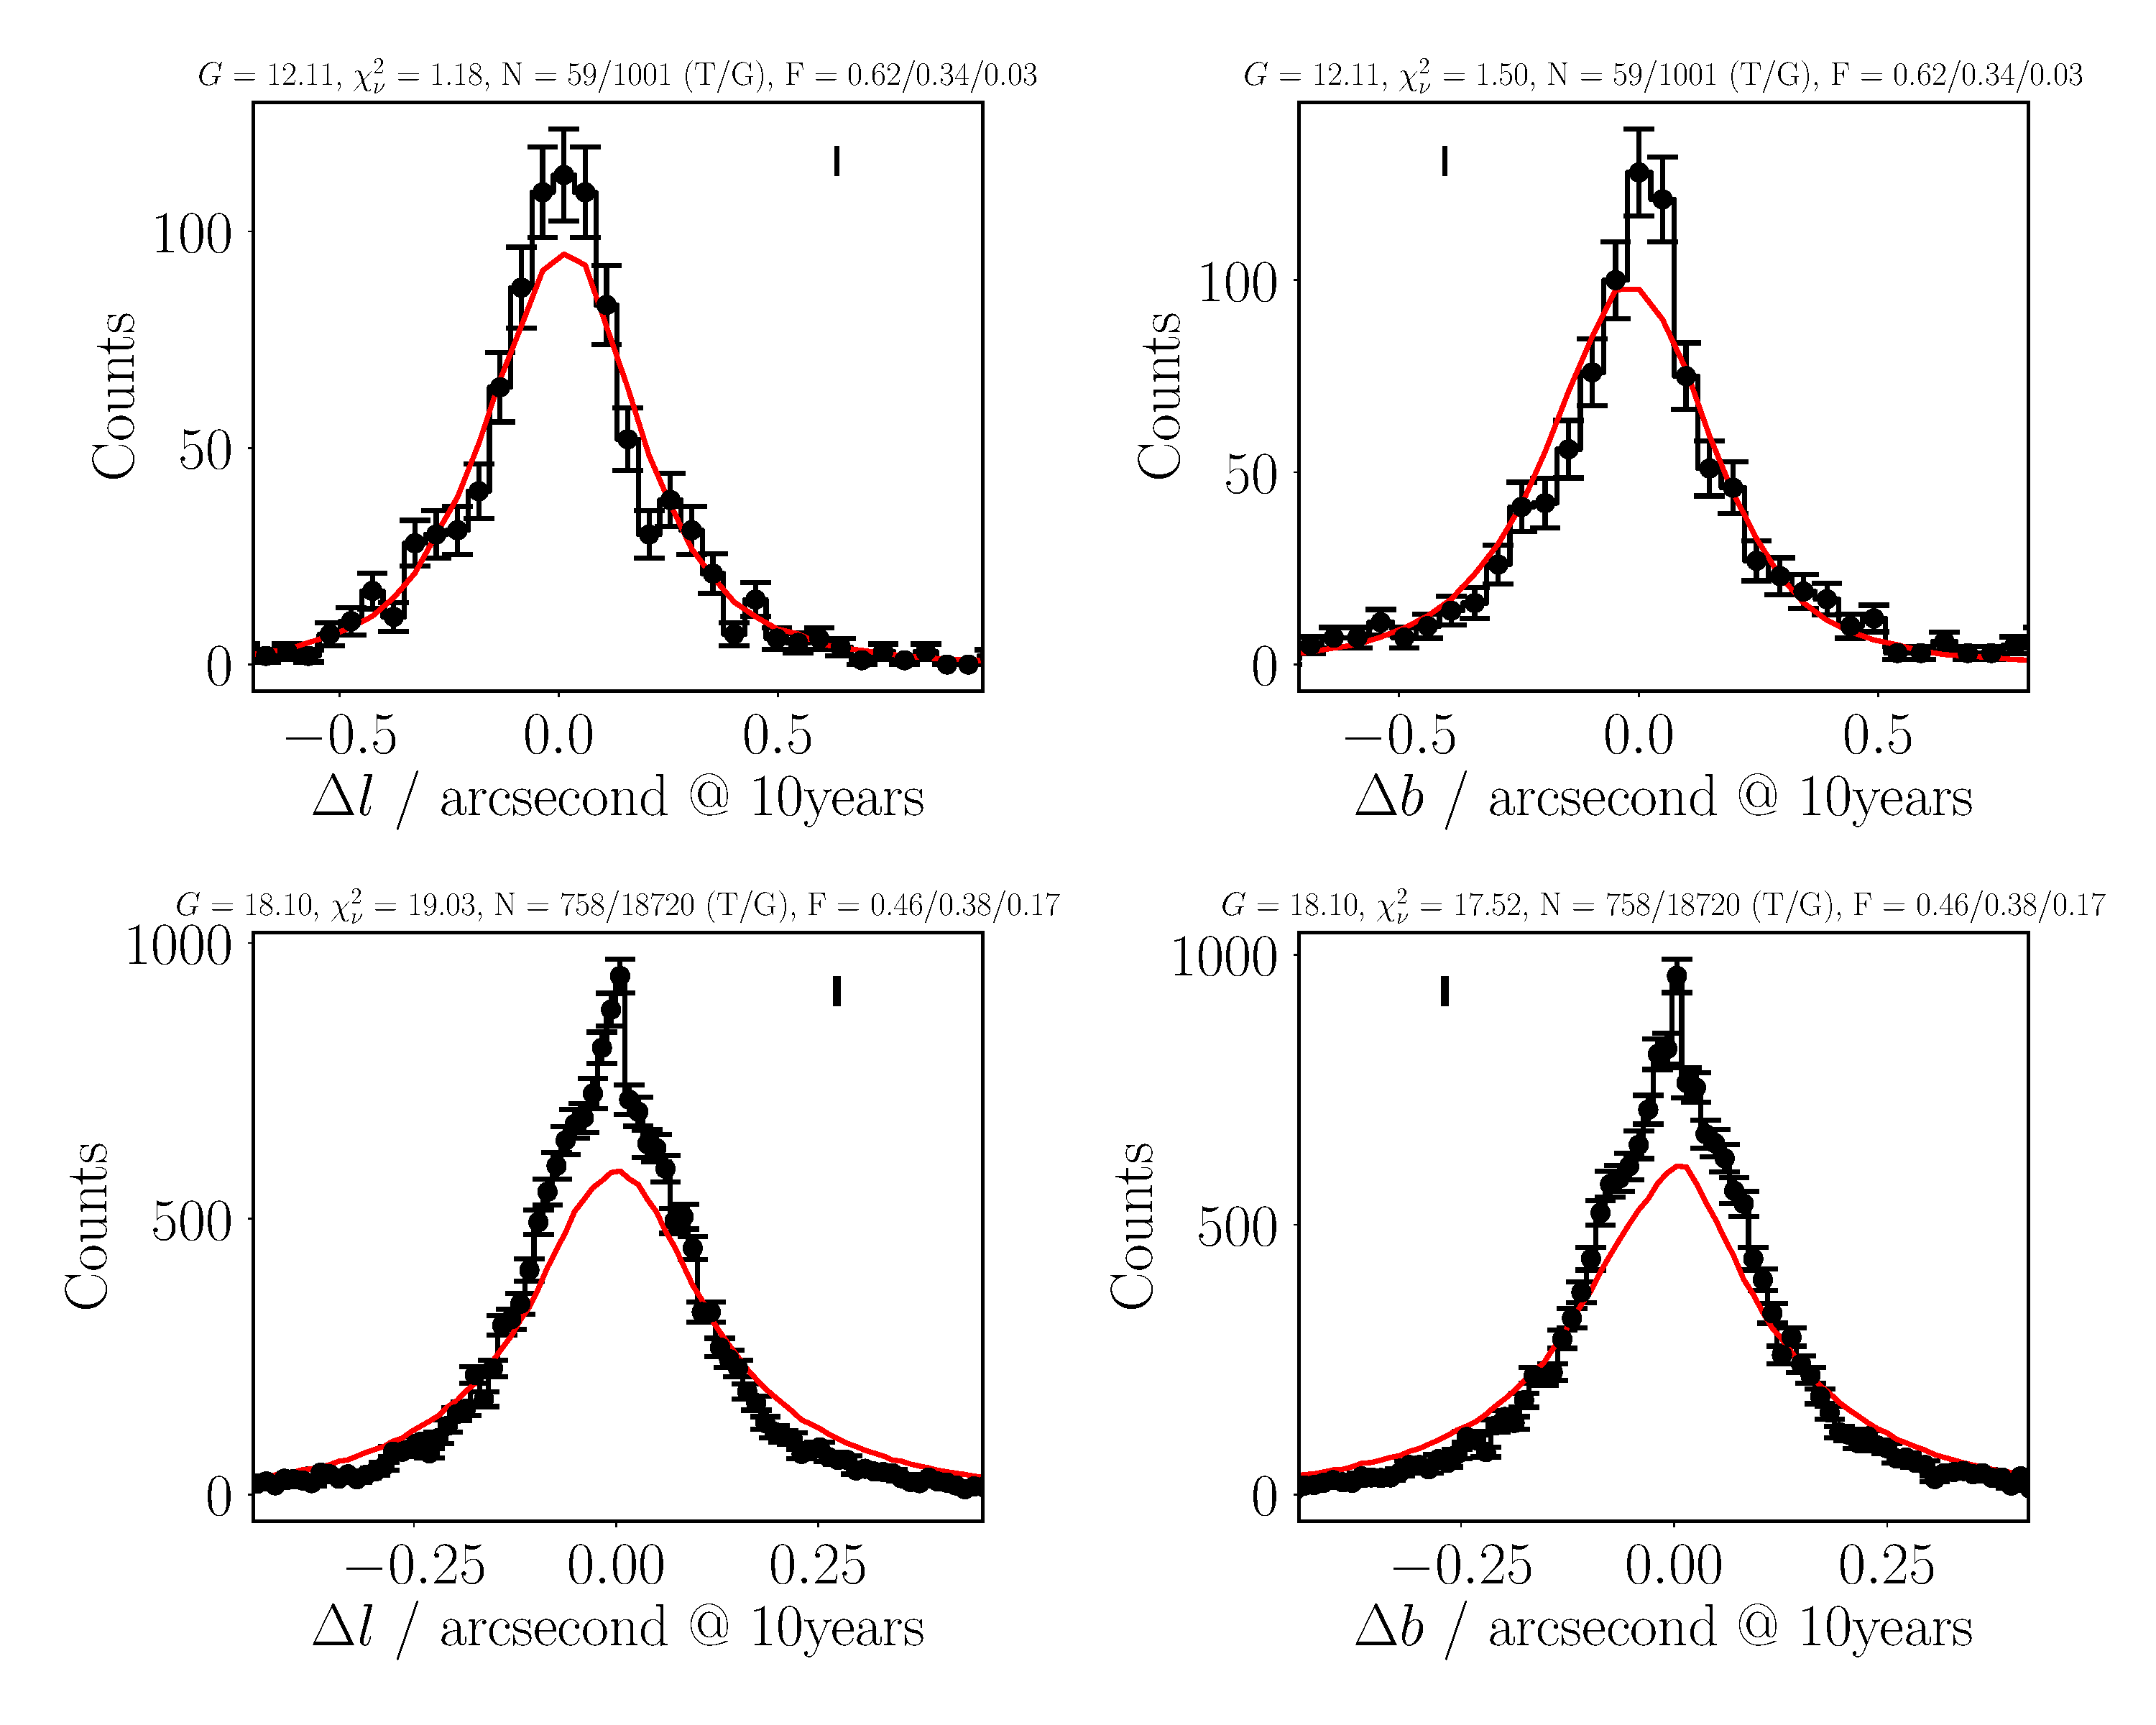
\includegraphics[width=\columnwidth]{Plots/plots_pm_gaia_180_85.pdf}
    \caption{Proper motions in Galactic coordinates (longitude, left column, and latitude, right column) for \textit{Gaia} $G = 12$ (top row) and $G=18$ (bottom row) for the Galactic north pole $b \geq 80^\circ$. Black errorbars are \textit{Gaia} proper motions, with red line our simulated distribution of proper motions using TRILEGAL. Small errorbar in the corner of each subfigure represents the average uncertainty of the \textit{Gaia} proper motions in the given subsample.}
    \label{fig:polepmcomp}
\end{figure}

In all cases discussed in this section, we will compare the \textit{Gaia} and model proper motions in Galactic coordinates, converted to an absolute positional shift on a 10-year baseline; units of $\mathrm{mas}\,\mathrm{year}^{-1}$ are therefore converted by a factor of 100. The \textit{Gaia} proper motions are rotated from their equatorial proper motions via the \texttt{astropy} (some citation for astropy here) \texttt{SkyCoord} framework. In practice, we would likely subsequently have to convert our Galactic frame proper motions to equatorial proper motions, which could be achieved as detaled by the \textit{Gaia} documentation\footnote{Details on the coordinate transforms between Galactic and ICRS frames for positions, proper motions, and five-parameter uncertainty propagation can be found \href{https://gea.esac.esa.int/archive/documentation/GDR2/Data_processing/chap_cu3ast/sec_cu3ast_intro/ssec_cu3ast_intro_tansforms.html}{here}.}; see Appendix for a brief description of how we perform this coordinate frame rotation from the Galactic coordinates our model is computed in, into equatorial coordinates. Note also that we have convolved our model distributions with the typical uncertainty of the \textit{Gaia} sources' proper motions, to ensure that the two compare more fairly in cases of non-negligible uncertainty at the faint magnitudes. This average proper motion uncertainty is shown as an errorbar in the corner of the corresponding figures that accompany the following sections.

\begin{figure}
    \centering
    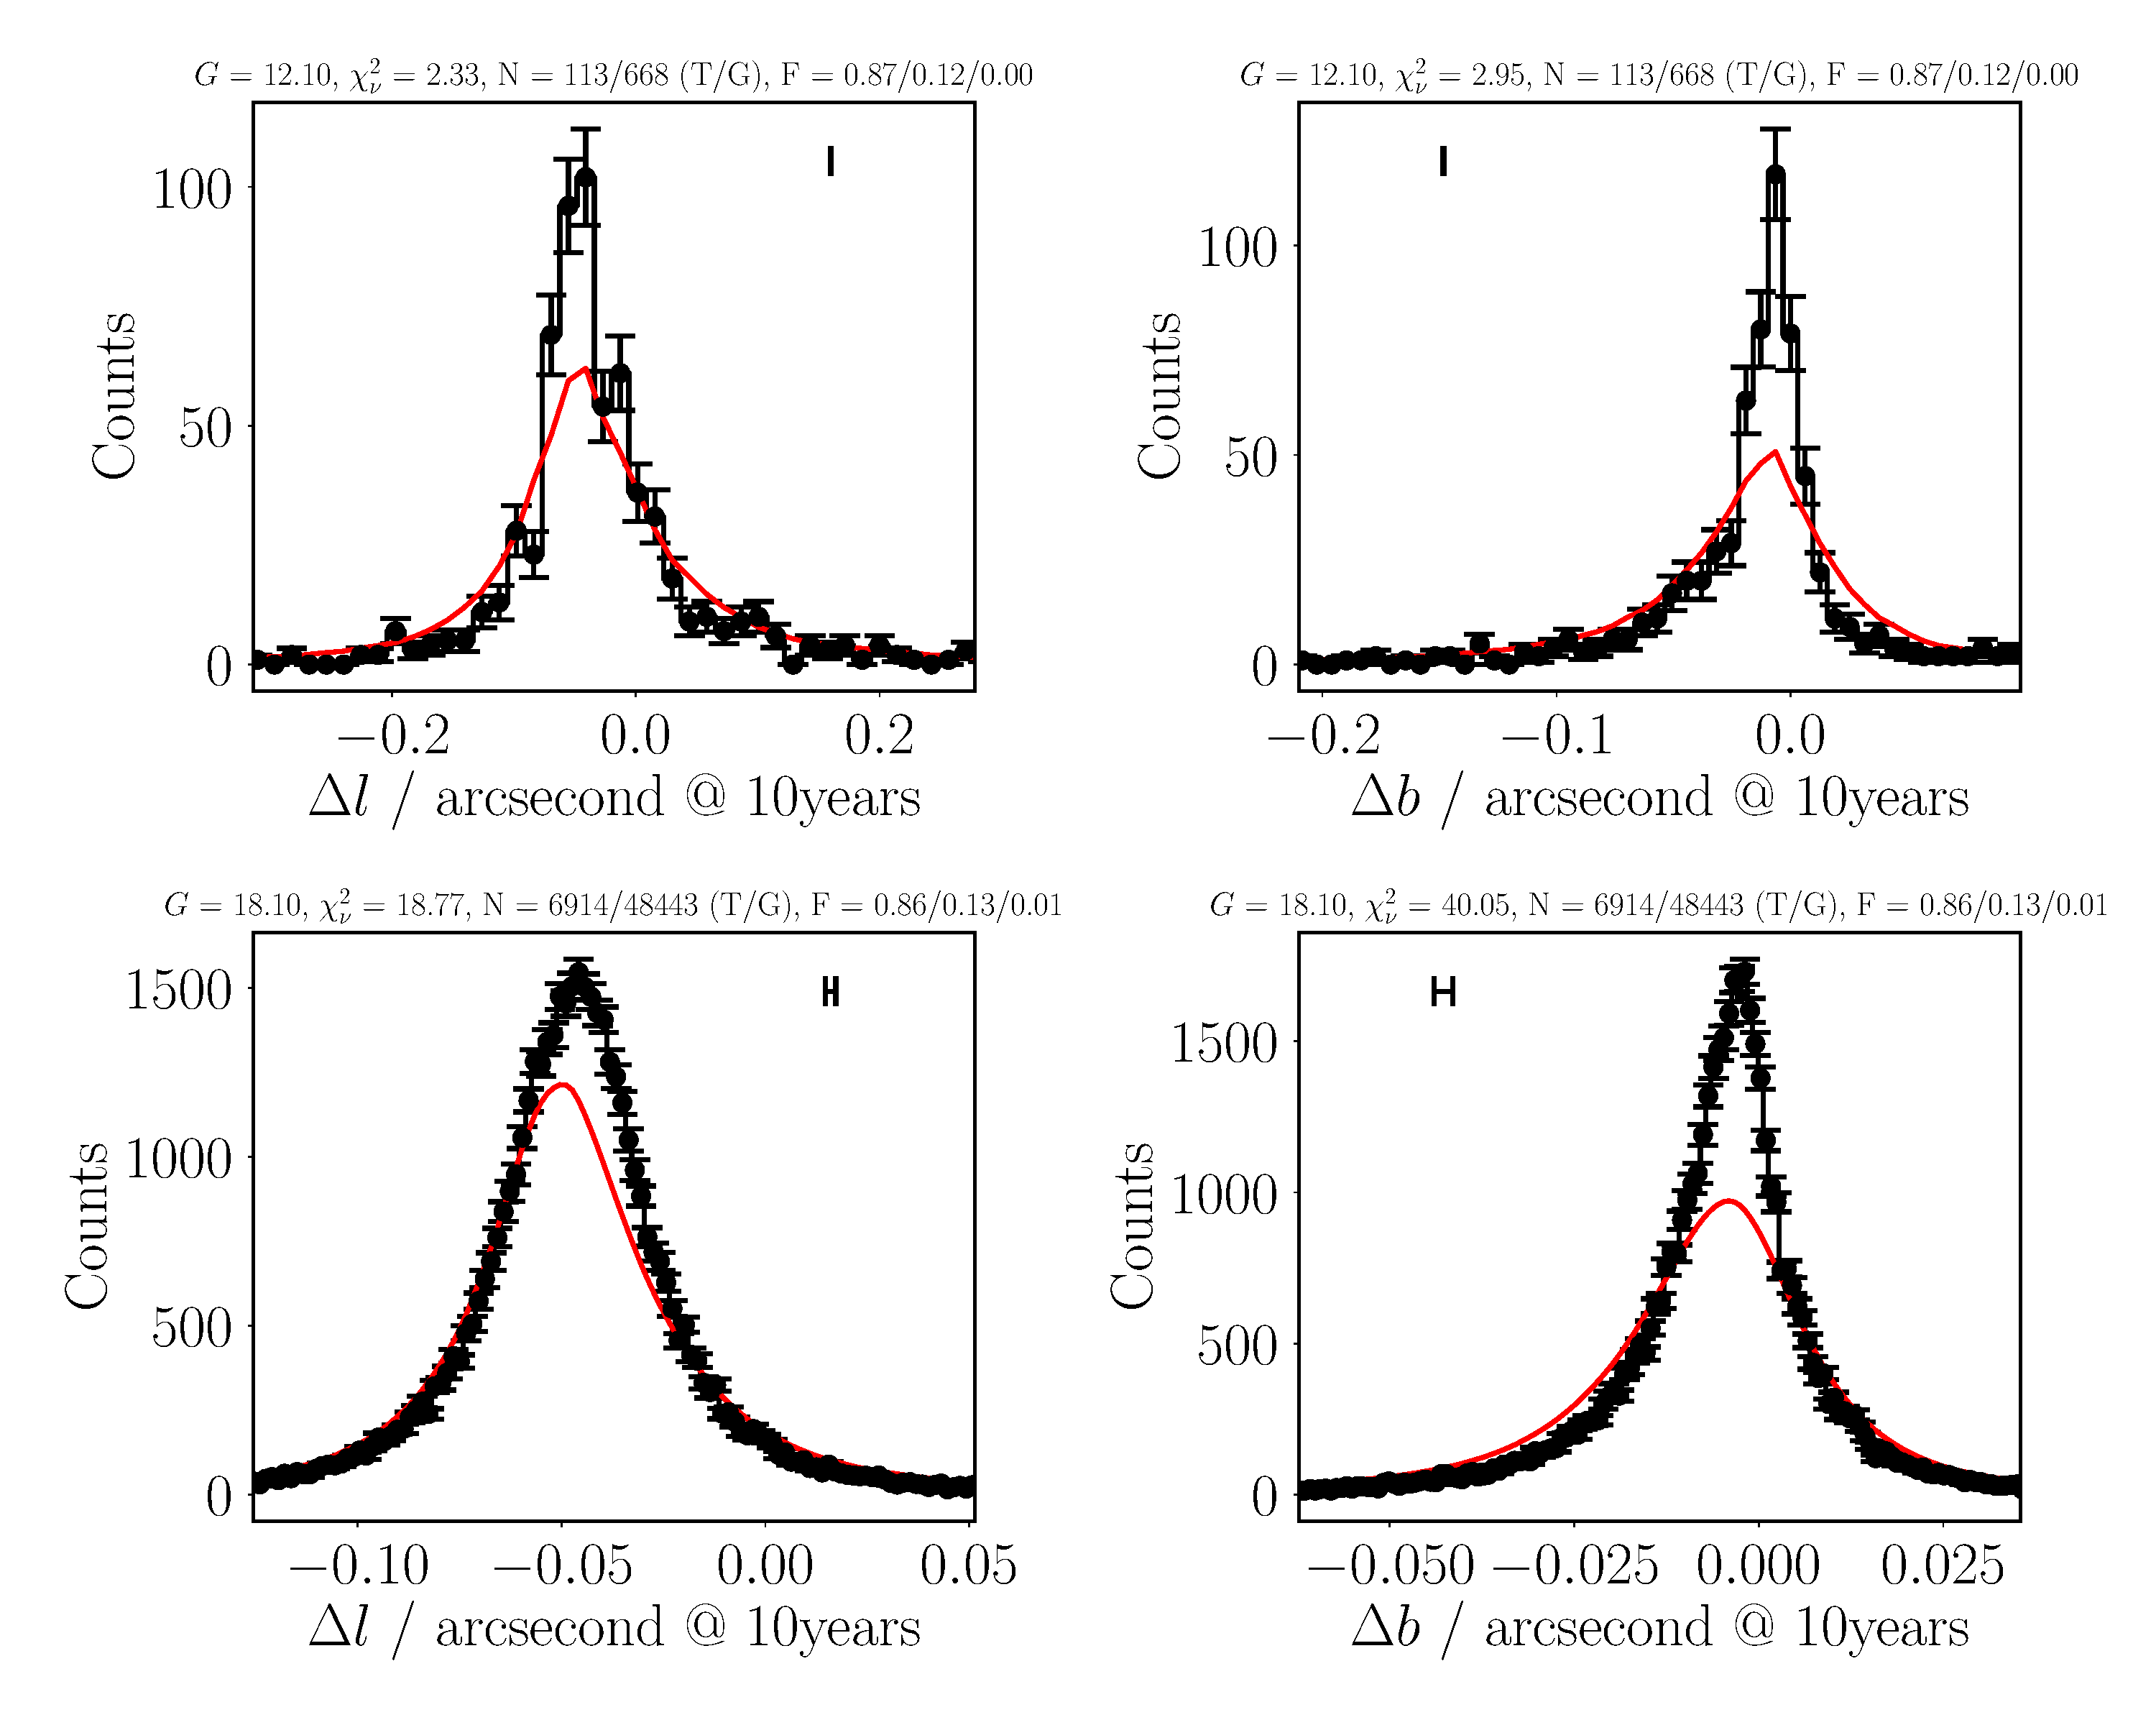
\includegraphics[width=\columnwidth]{Plots/plots_pm_gaia_90_0.pdf}
    \caption{Proper motions in Galactic coordinates for a sightline along the positive $y$ axis, towards $l = 90^\circ$, $b = 0^\circ$. Subfigures and lines are the same as in Figure \ref{fig:polepmcomp}.}
    \label{fig:l90comp}
\end{figure}

\subsection{Galactic Poles}
The Galactic poles probe a "top-down" view of the Galaxy, with significant contribution from the halo. Here we see (Figure \ref{fig:polepmcomp}) good agreement at a small range of bright ($G=12$) and faint ($G=18$) magnitudes ($\Delta G = 0.2$), for $b \geq 80^\circ$. The central, mean offset is in good agreement, and the dispersion agrees well with the \textit{Gaia} distribution. We see a slight discrepancy in the number of zero-proper motion objects, which affect the relative counts at other offsets (with the model curve normalised to the \textit{Gaia} counts), which is likely caused by the contamination of the Galactic sources by extragalactic objects, which we do not remove from the data in any way.

As we also get incredibly similar results at the Galactic south pole for $b \leq 75^\circ$, we conclude that the model works well when viewing sources out-of-plane, where the radial and tangential components are the dominant terms.

\subsection{The $y$ Axis}
Another comparison we can make is to look directly down the $y$ axis, at either $l = 90^\circ$ or $l = 270^\circ$, shown for the $+y$ direction, at $l = 90^\circ$, in Figure \ref{fig:l90comp}. Here we also see broad qualitative agreement between the data and model, with the bright subsample showing a slightly tighter distribution of offsets in the data than our model, although a reduced chi-squared of 2.4 suggests this is in part due to low number statistics, and the two are not particularly at odds with one another. In the faint sample we see broad agreement, although a slight tension with the clustering at the peak; however, as we only require a sense of the \textit{spread} of the unknown proper motions (as well as a rough estimate of the average of the distribution), we are not unduly concerned by such disparities. The opposing view -- along $-y$ -- shows essentially the same distribution as the view towards $l = 90^\circ$, just with the asymmetry in the tails of the distribution flipped in sign, as should be expected when looking towards or away from the Galactic rotation with increasing distance.

\begin{figure}
    \centering
    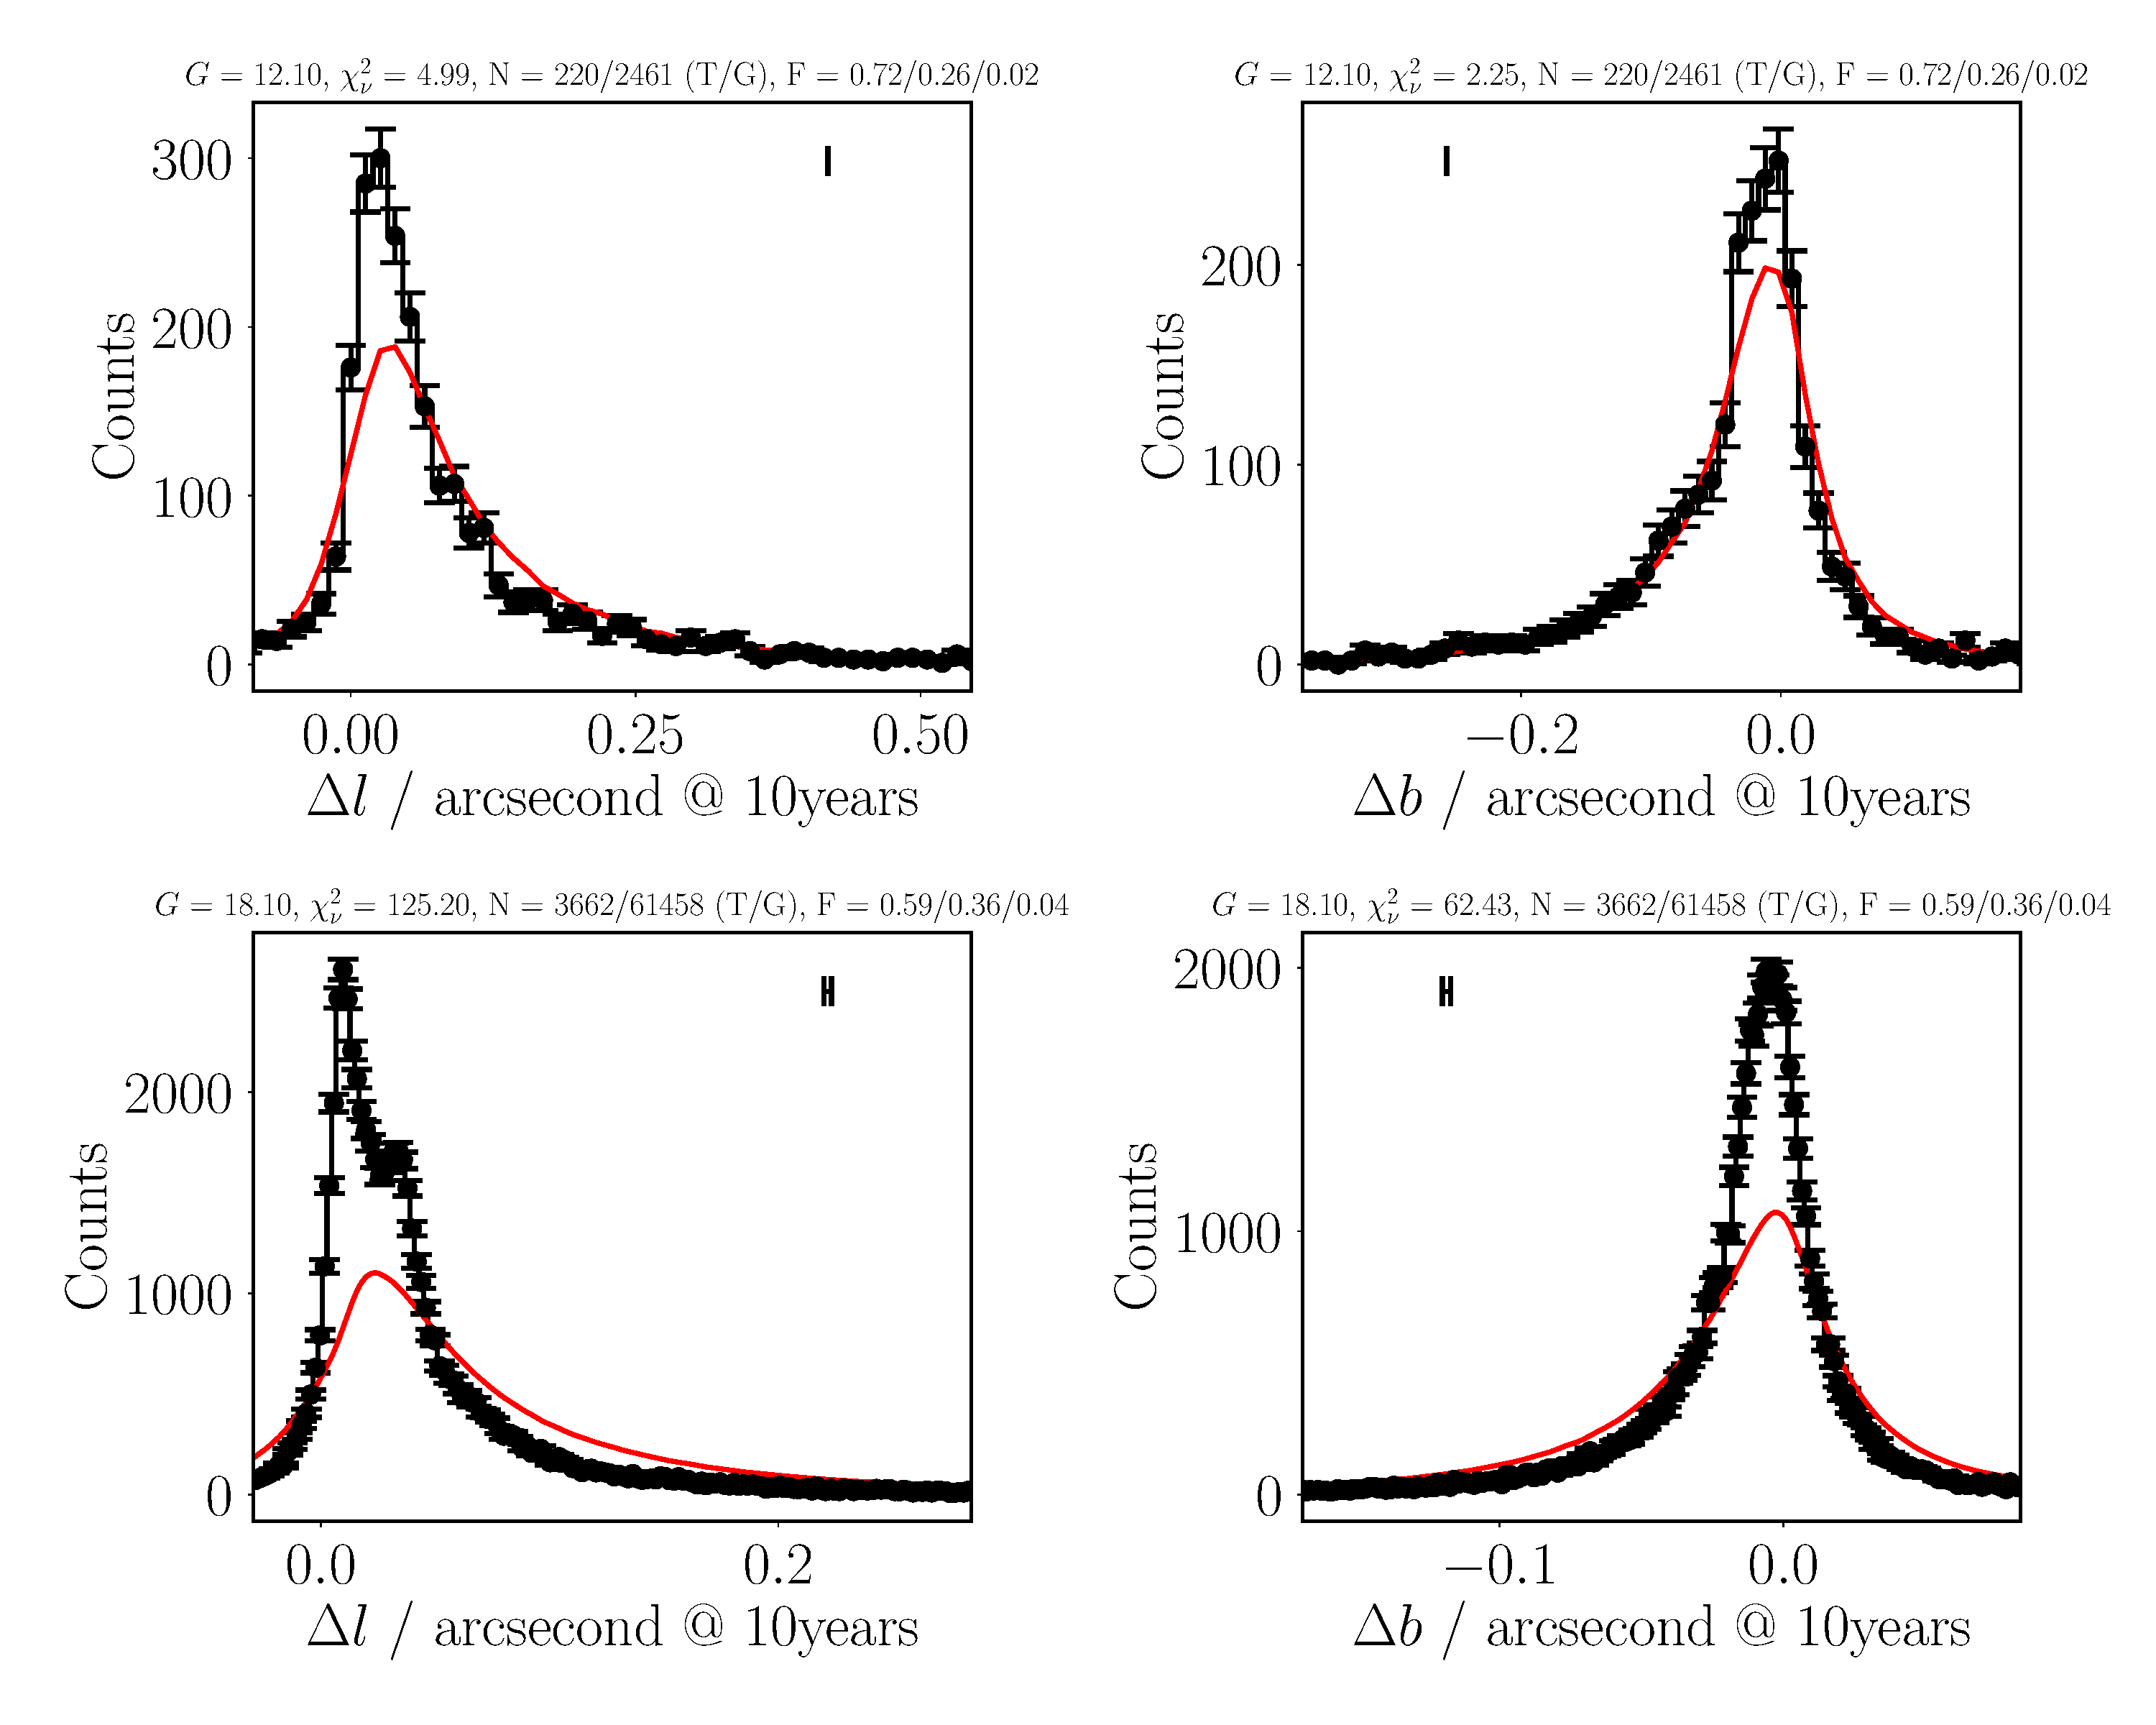
\includegraphics[width=\columnwidth]{Plots/plots_pm_gaia_180_20.pdf}
    \caption{Proper motions in Galactic coordinates for a sightline towards $l = 180^\circ$, $b = 20^\circ$. Subfigures and lines are the same as in Figure \ref{fig:polepmcomp}.}
    \label{fig:l180comp}
\end{figure}

\subsection{The Galactic Anti-Center}
Here we can consider another orthogonal axis in the Galactic rotation, with simplified Oort constant motions; the Galactic anti-center, at $l=180^\circ$; here, however, we also consider a slightly out-of-plane angle, with our sightline centered on $b = 20^\circ$. This distribution, for our bright and faint sub-sample, can be seen in Figure \ref{fig:l180comp}.

Here we see slightly less agreement between our model and the \textit{Gaia} data. We believe this is, at least in part, again caused by our out-of-plane viewing angle, which is causing a visible number of extragalactic, zero proper motion objects to be present in our data at faint magnitudes in the galactic longitude offsets; we assume a similar effect is likely present in the latitude data, as well. We are reassured, once again, that our dispersion (and its relative lengthscales in the positive and negative directions) and approximate peak offset are in rough agreement with the data, albeit with some caveats.
\begin{figure}
    \centering
    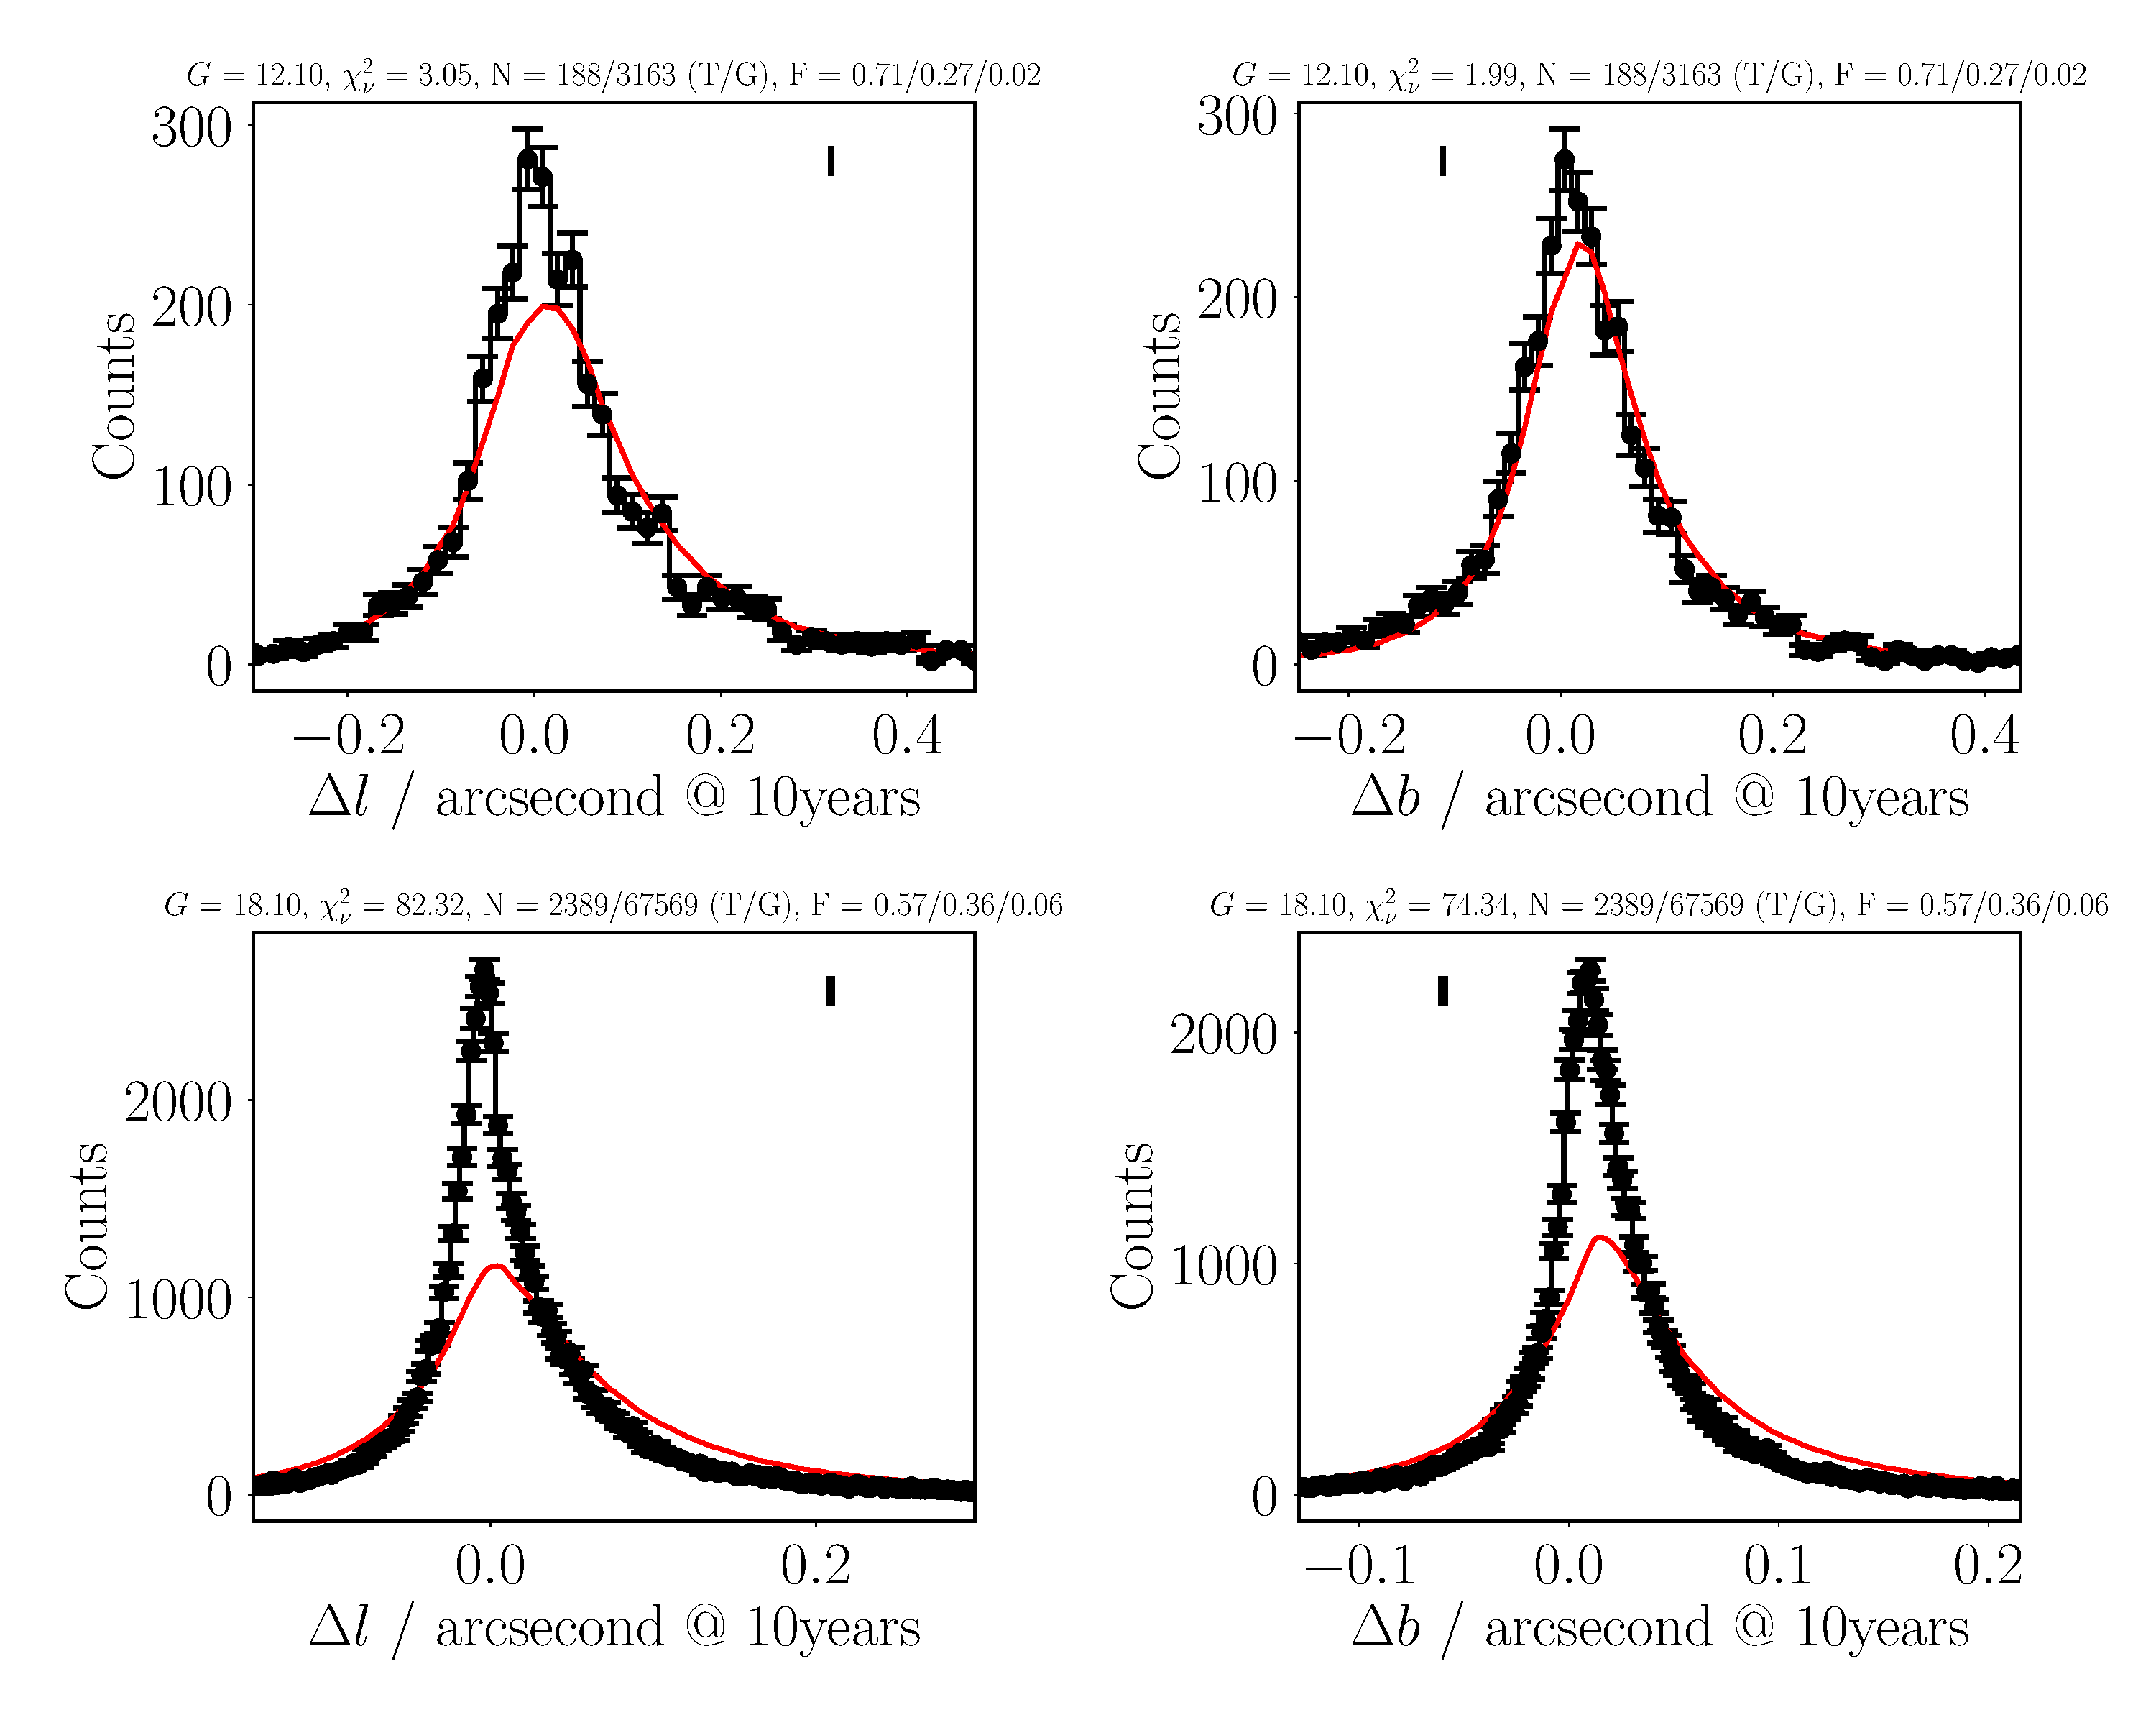
\includegraphics[width=\columnwidth]{Plots/plots_pm_gaia_220_-30.pdf}
    \caption{Proper motions in Galactic coordinates for a sightline towards $l = 220^\circ$, $b = -30^\circ$. Subfigures and lines are the same as in Figure \ref{fig:polepmcomp}.}
    \label{fig:l220comp}
\end{figure}

\subsection{$l = 220^\circ$, $b = -30^\circ$}
All previous sightlines were ``convenient'' viewing angles; they simplified the various components that make the Galactic longitude or latitude proper motion projections, in cosine or sine cancellations of sky coordinates in some fashion or in which component is responsible for the latitudinal proper motion. Here we show a somewhat more ``arbitrary'' sightline in the Galaxy, with an ``uneven'' cosine sine projection factor, in Figure \ref{fig:l220comp}.

Once again, we are unfortunately potentially contaminated by extragalactic sources, being out of the plane once again, which may slightly contribute to the more peaked distribution in very low proper motion objects. However, as we are only looking for broad, qualitative agreement (albeit across all sightlines), we are relatively happy with this distribution comparison once again, with dispersions, asymmetries in the dispersions, and rough maximum in offset all in agreement across the magnitude range of the data.

\begin{figure}
    \centering
    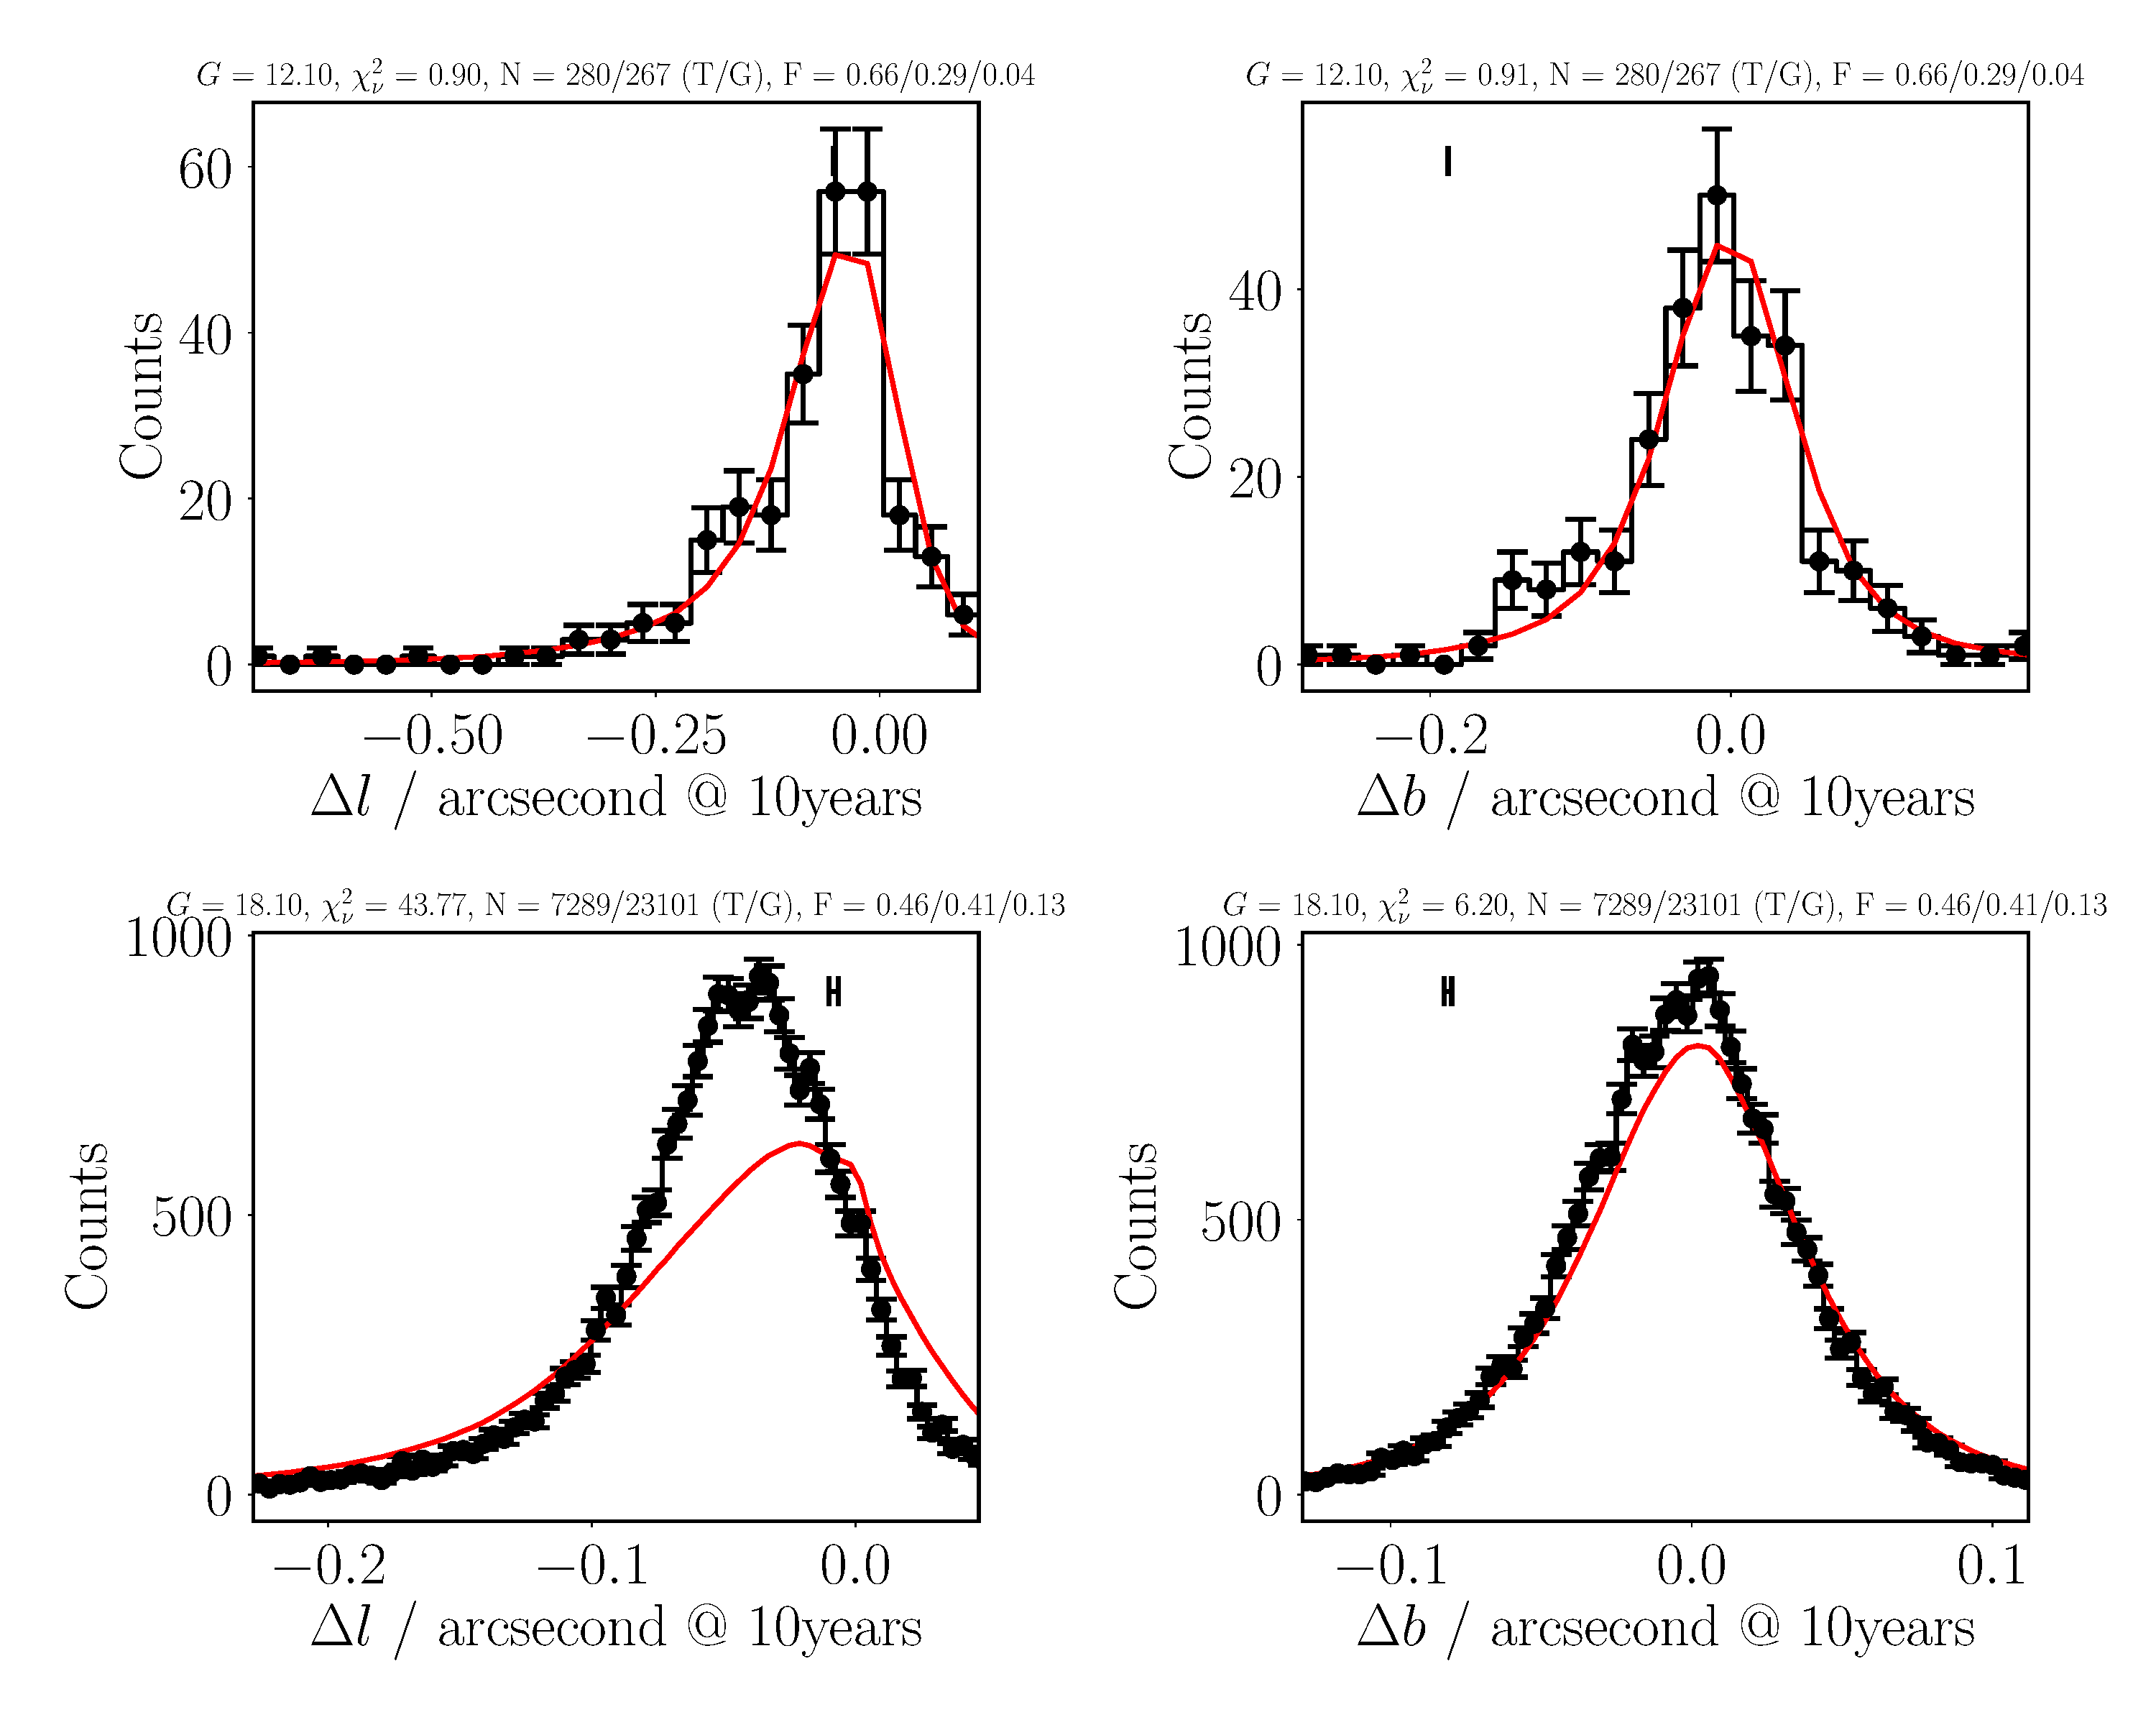
\includegraphics[width=\columnwidth]{Plots/plots_pm_gaia_0_20.pdf}
    \caption{Proper motions in Galactic coordinates for a sightline towards $l = 0^\circ$, $b = 20^\circ$. Subfigures and lines are the same as in Figure \ref{fig:polepmcomp}.}
    \label{fig:l0comp}
\end{figure}

\subsection{The Galactic Center}
With rough agreement in all other directions, we can now consider the final angle of comparison undertaken: the Galactic center. Looking towards the bulk of the Galaxy, these sightlines are the most potentially subject to discrepancies in our model. Here we have broken the sightline into three viewing angles: towards the Galactic center, but out of the plane ($l = 0^\circ$, $b = 20^\circ$), and two sightlines 30 degrees offset in either direction, but in the plane ($l = 30^\circ$, $b = 0^\circ$; $l = 330^\circ$, $b = 0^\circ$).

\subsubsection{$l = 0^\circ$, $b = 20^\circ$}
The viewing angle towards the $x$ axis is shown, for the two subsamples of magnitude ranges, in Figure \ref{fig:l0comp}. Here, at bright magnitudes, we have good agreement between both Galactic longitude and latitude distributions. However, at faint magnitudes, we only see good agreement in the latitudinal component. For longitudinal proper motion shifts there is an extra ``bump'' in offsets at larger negative values for the \textit{Gaia} data than our model produces.

\begin{figure}
    \centering
    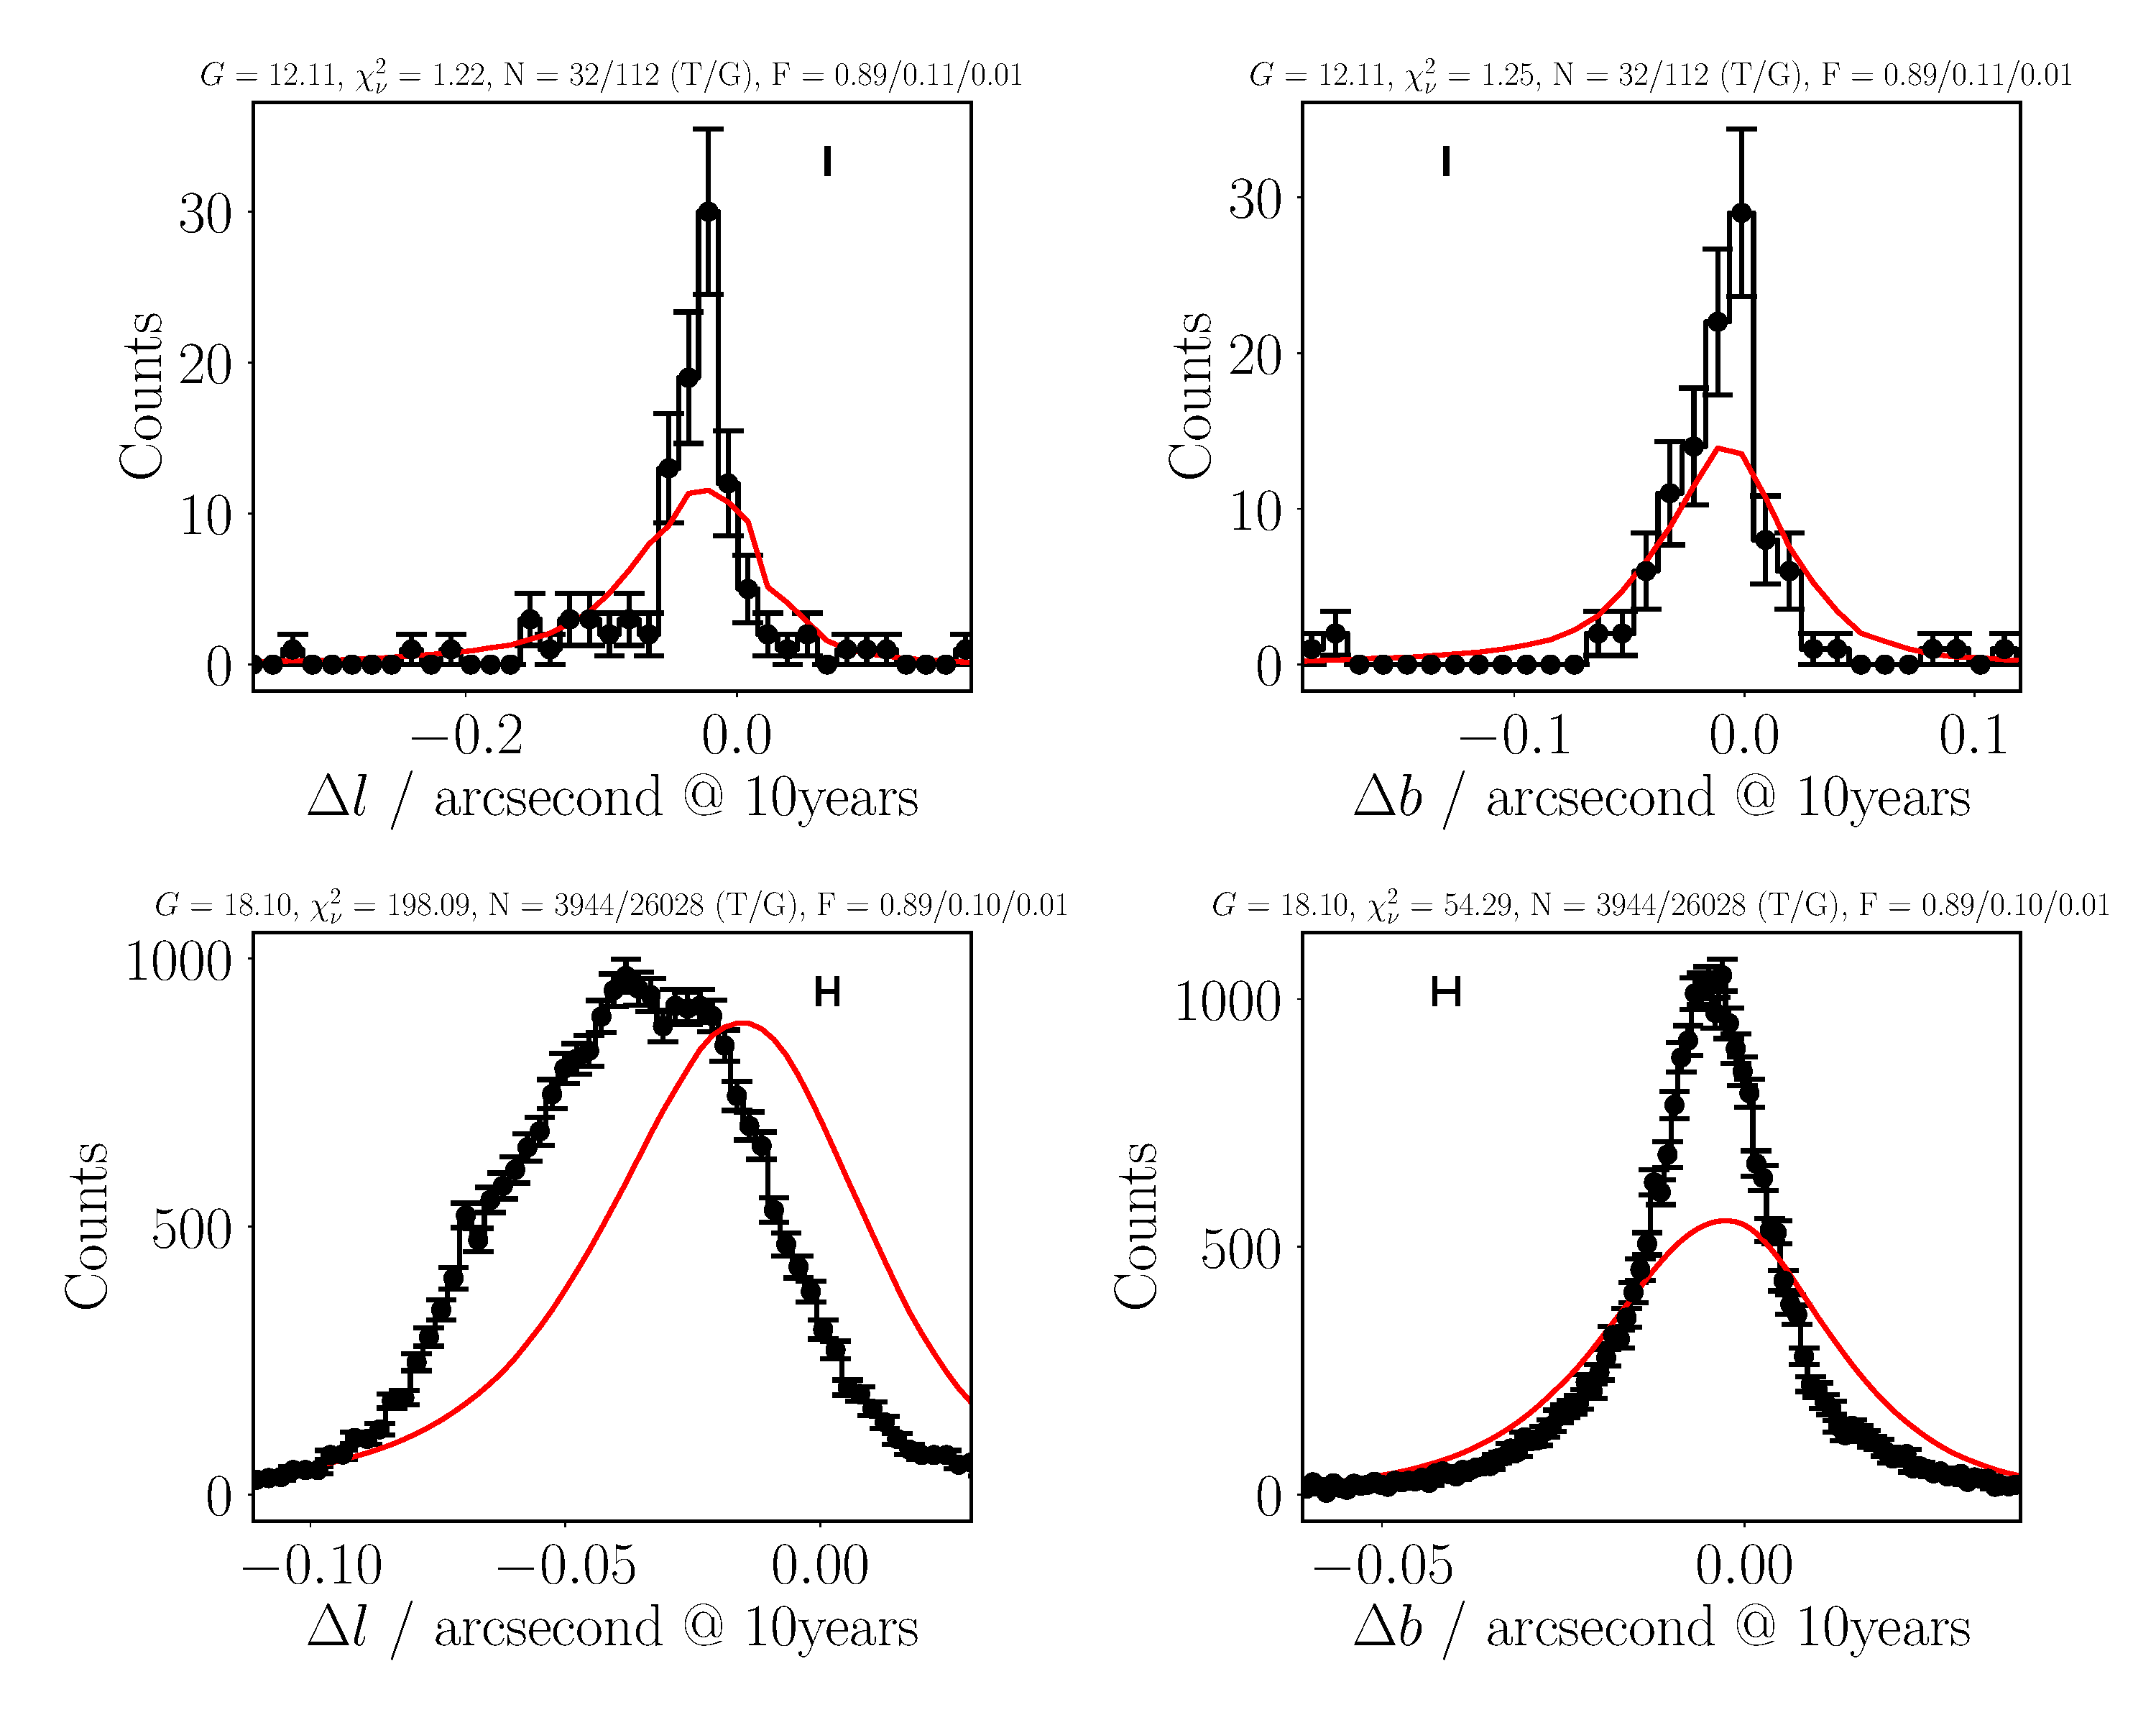
\includegraphics[width=\columnwidth]{Plots/plots_pm_gaia_30_0.pdf}
    \caption{Proper motions in Galactic coordinates for a sightline towards $l = 30^\circ$, $b = 0^\circ$. Subfigures and lines are the same as in Figure \ref{fig:polepmcomp}.}
    \label{fig:l30comp}
\end{figure}

\subsubsection{$l = 30^\circ$, $b = 0^\circ$}
Figure \ref{fig:l30comp} shows the distribution of bright and faint samples of proper motion offsets slightly off from the Galactic center, towards $l = 30^\circ$. Here we see an \textit{acceptable} distribution of proper motions for the $G = 12$ sample, with $\chi_\nu^2 \simeq 1.2$ in both orthogonal directions, but perhaps supported by low number statistics easing any issues with the underlying distributions. The faint sample appears to be completely incompatible in either longitudinal or latitudinal directions: $\Delta b$ shows a much broader model distribution than the \textit{Gaia} data, and there appears to be a systematic offset in the $\Delta l$ proper motions. There is some potential bimodality in the \textit{Gaia} data that we do not see in our smooth model distribution.

As we currently cannot explain -- or accept -- these data as shown, we turn to the opposing sightline to verify the model in the symmetric rotation from the Galactic center.

\begin{figure}
    \centering
    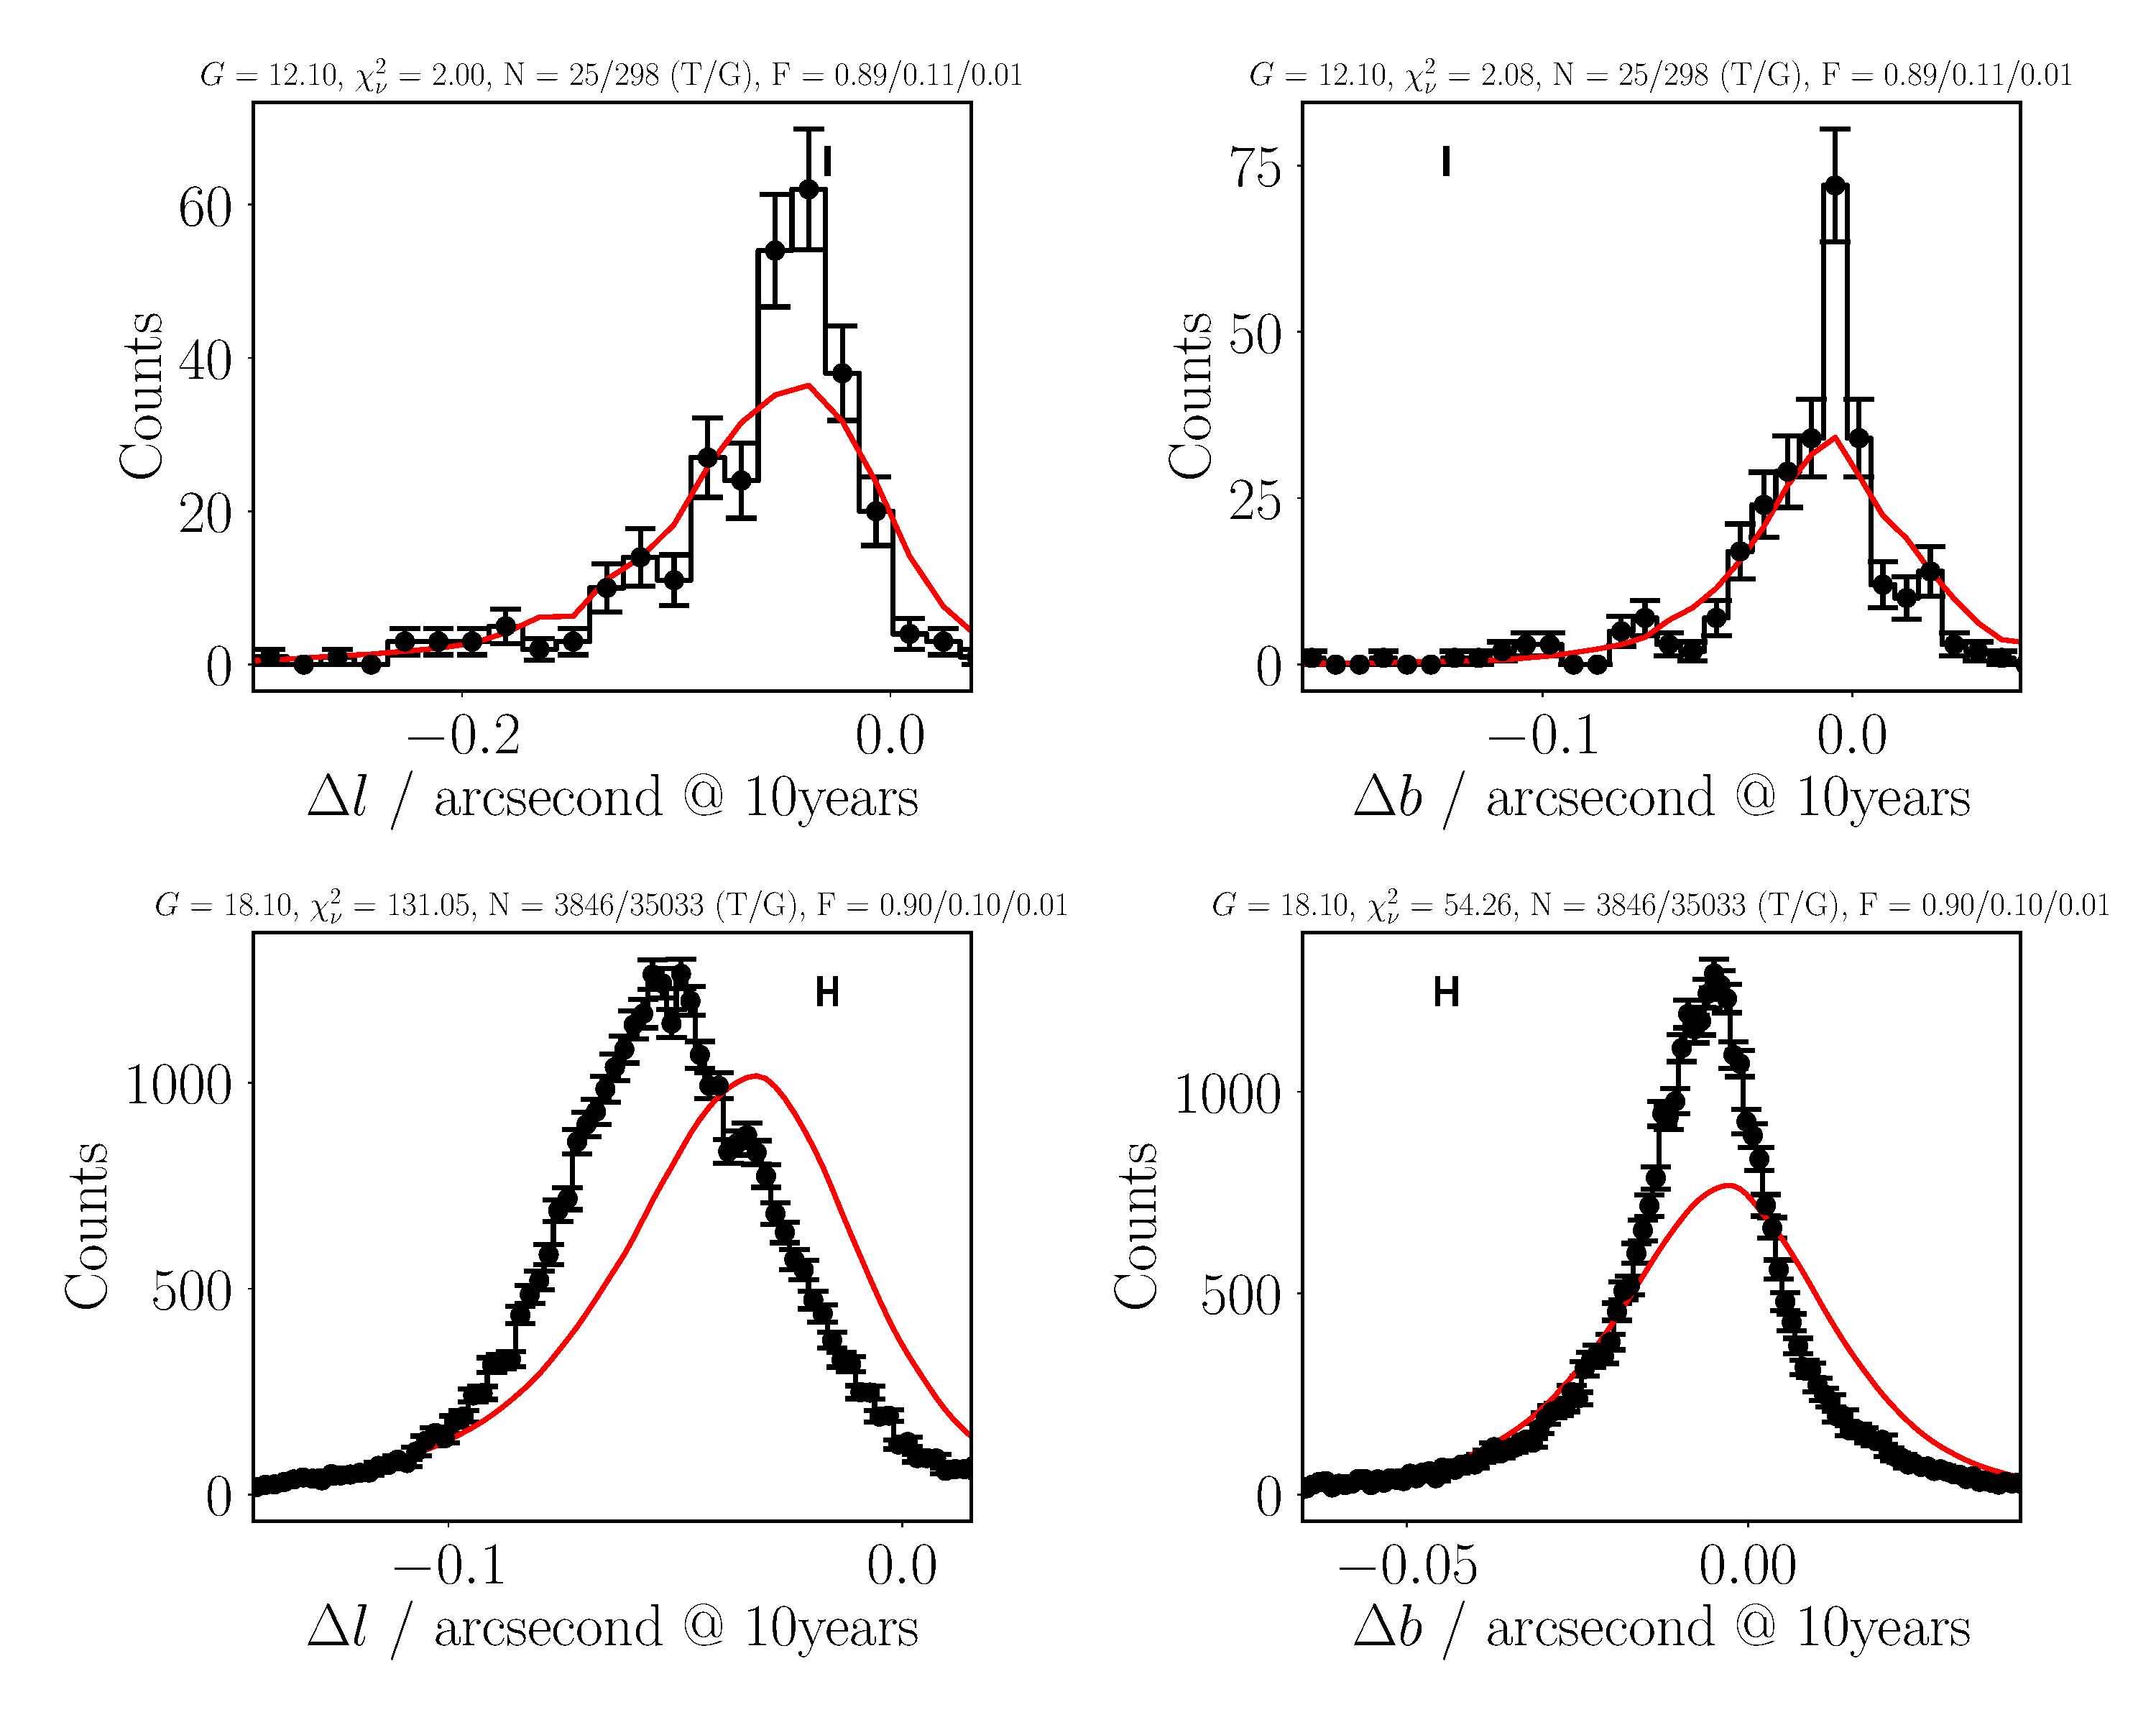
\includegraphics[width=\columnwidth]{Plots/plots_pm_gaia_330_0.pdf}
    \caption{Proper motions in Galactic coordinates for a sightline towards $l = 330^\circ$, $b = 0^\circ$. Subfigures and lines are the same as in Figure \ref{fig:polepmcomp}.}
    \label{fig:l330comp}
\end{figure}

\subsubsection{$l = 330^\circ$, $b = 0^\circ$}
The results for the $l = 330^\circ$ Galactic plane sightline are shown in Figure \ref{fig:l330comp}. These are qualitatively similar to those of the $l = 30^\circ$ sightline for both magnitude cuts and proper motion components. Thus, all descriptions from the above section apply: the bright sample shows reasonable agreement with lower number statistics, but the faint slice has a bimodal longitudinal distribution with an apparent average proper motion shift, and a poor dispersion in the latitudinal direction.

\section{Explaning the Model Disparity}
In the previous section we detailed a few example sightlines, which have varying levels of agreement between model and data. As the model works very well for some cases (the poles, the $y$ axis sightlines, and many other bright magnitude slices in other direction) but poorly in others (the faint Galactic center sightlines, to a lesser extent the Galactic anticenter or $l = 220^\circ$ direction), we must examine our data at another angle to make sense of these differences.

\begin{figure*}
    \centering
    \begin{subfigure}[b]{0.3\textwidth}
        \centering
        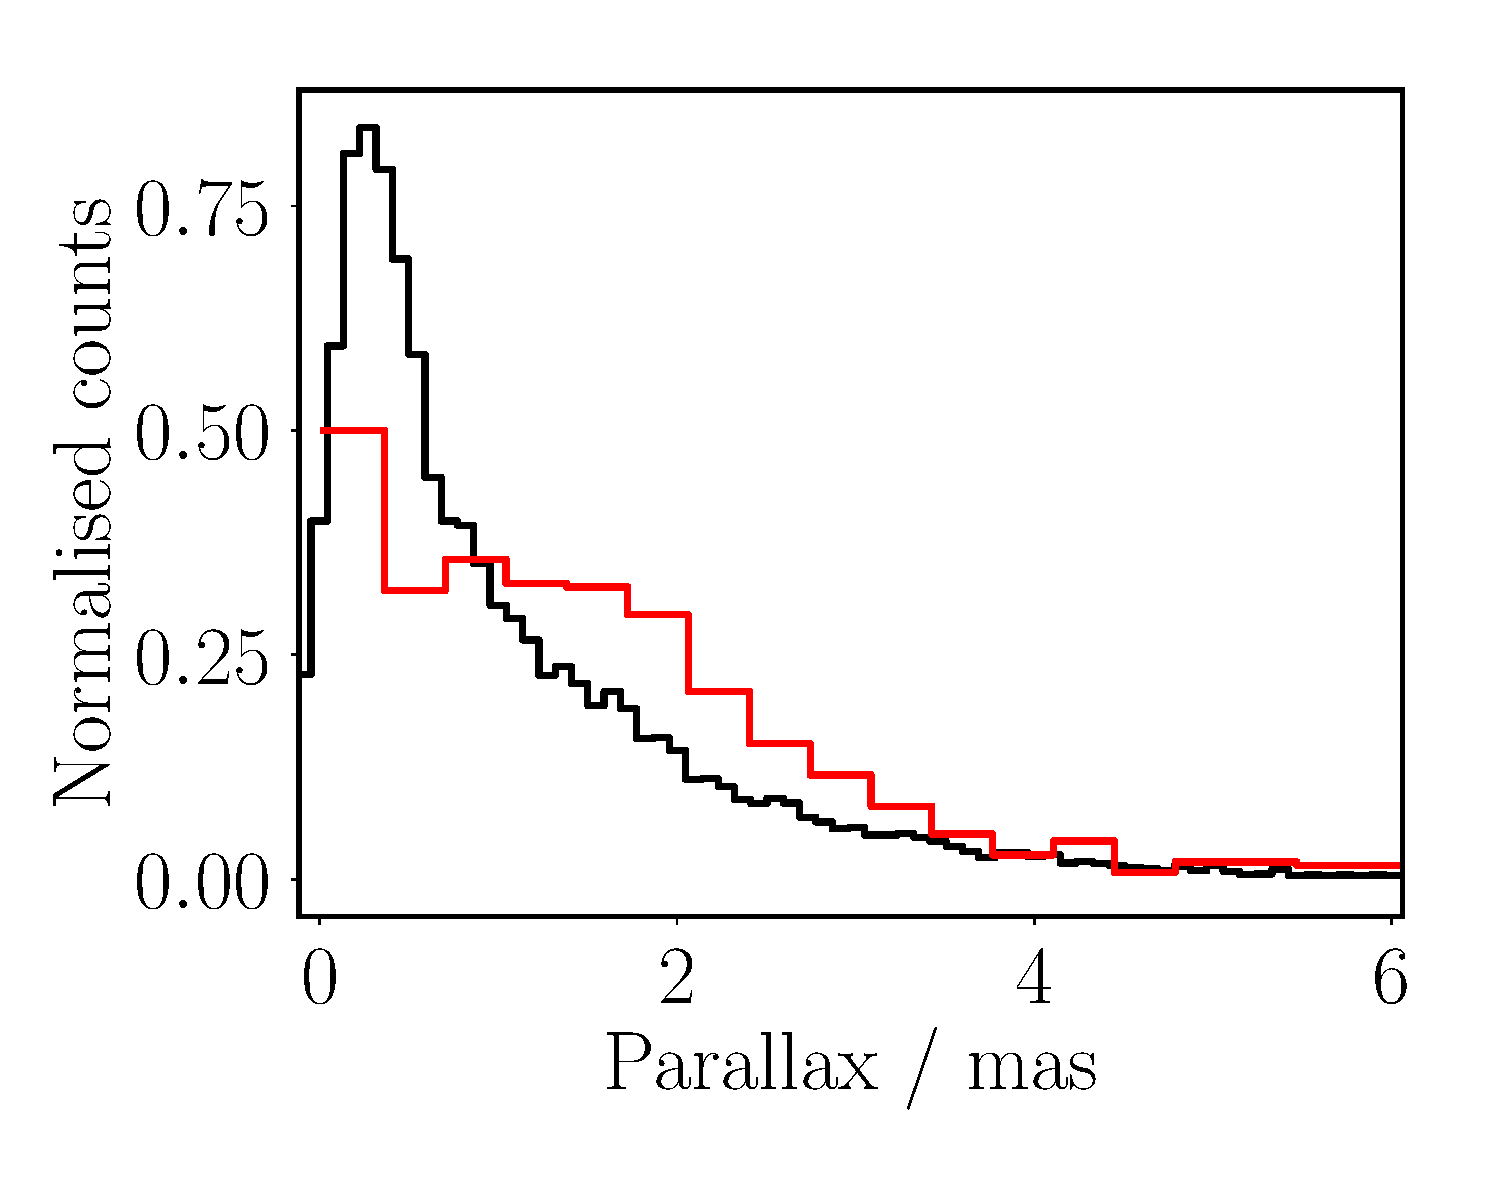
\includegraphics[width=\textwidth]{Plots/plot_dist_gaia_180_85_18.pdf}
        \caption{Parallaxes at the Galactic north pole, $b \geq 80^\circ$.}
        \label{fig:NGPdist}
    \end{subfigure}
    \begin{subfigure}[b]{0.3\textwidth}
        \centering
        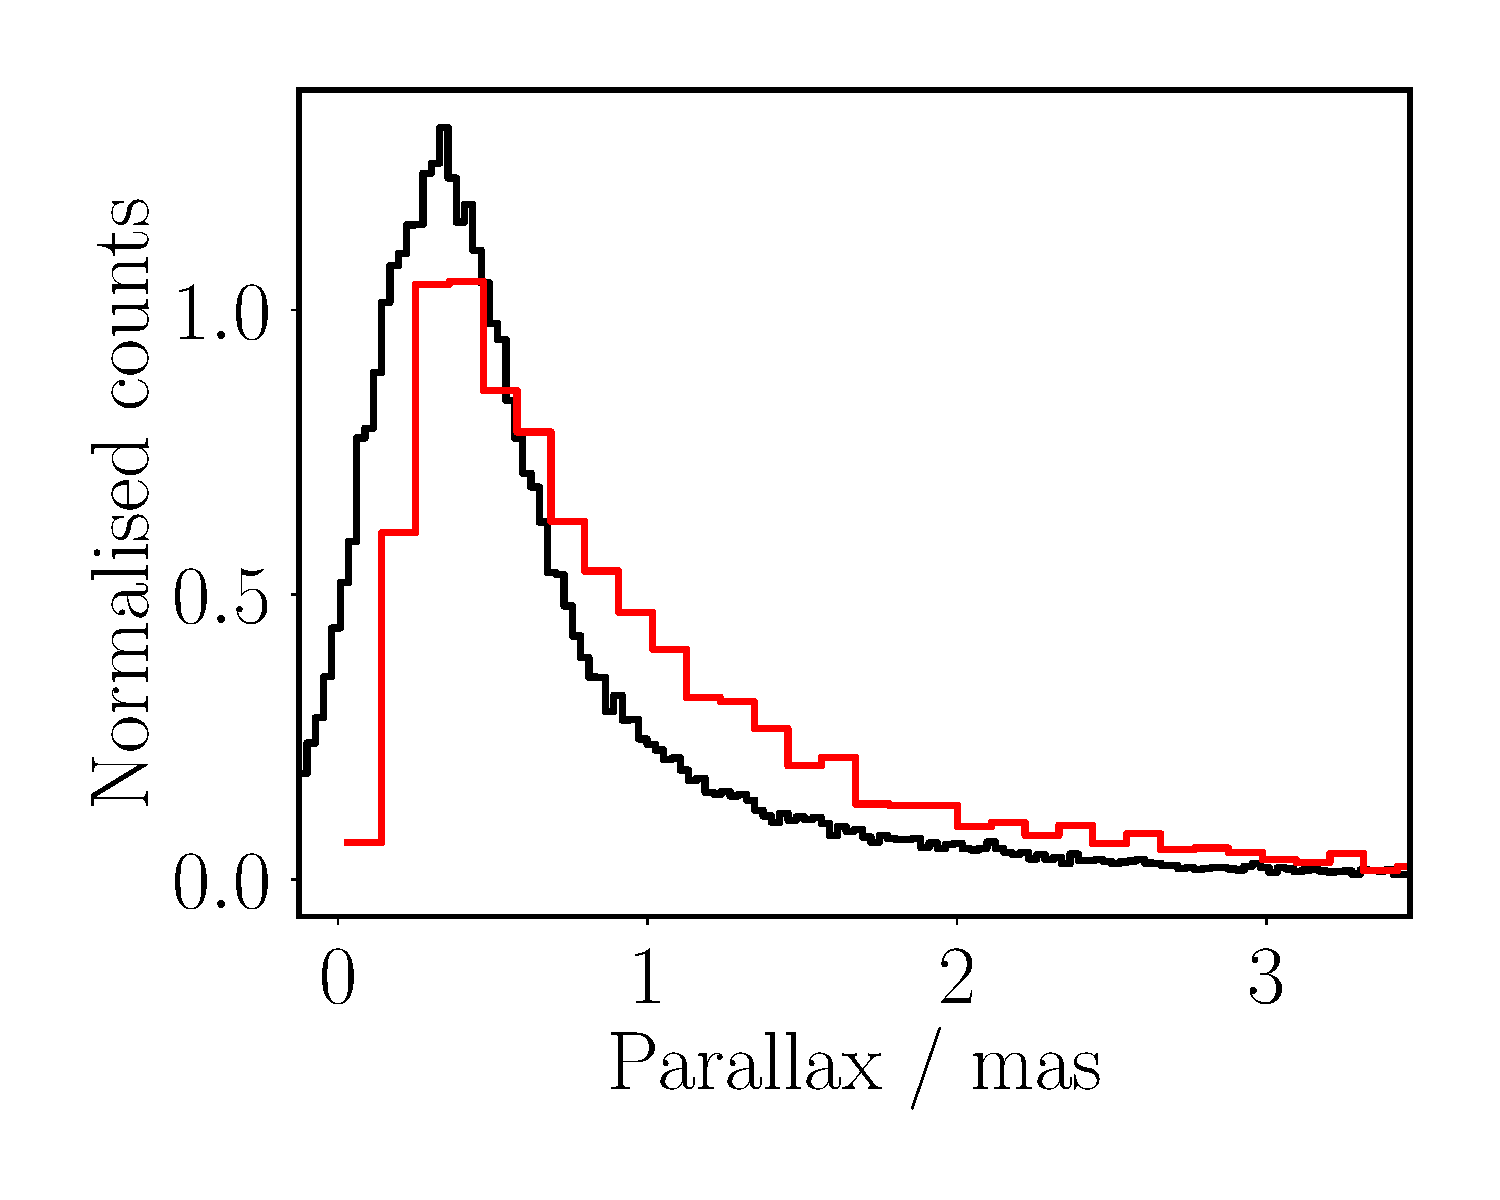
\includegraphics[width=\textwidth]{Plots/plot_dist_gaia_180_20_18.pdf}
        \caption{Parallaxes at the Galactic anti-center, $l = 180^\circ$, $b = 20^\circ$.}
        \label{fig:l180dist}
    \end{subfigure}
    \begin{subfigure}[b]{0.3\textwidth}
        \centering
        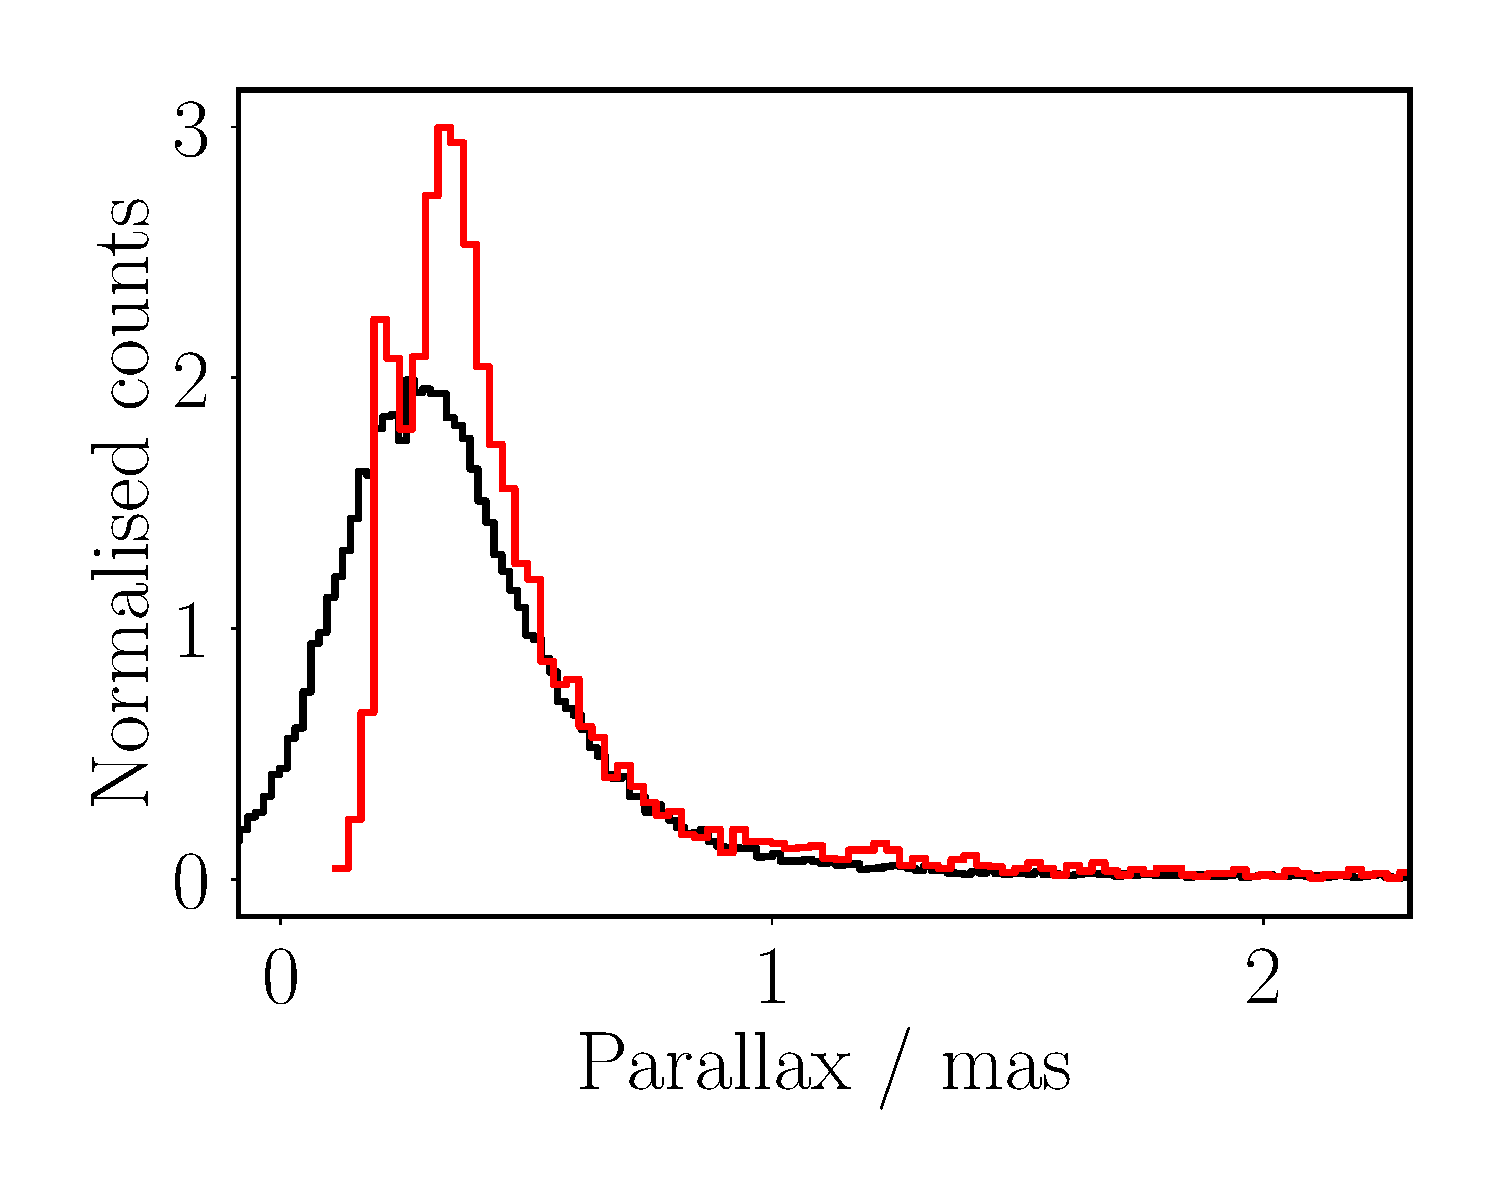
\includegraphics[width=\textwidth]{Plots/plot_dist_gaia_90_0_18.pdf}
        \caption{Parallaxes looking towards $+y$, $l = 90^\circ$, $b = 0^\circ$.}
        \label{fig:l90dist}
    \end{subfigure}
    \caption{Distributon of measured parallaxes to objects in the \textit{Gaia} sample at $G = 18$ (black histogram) and inverted distances from absolute distance modulus from a TRILEGAL simulation (red histogram).}
    \label{fig:goodishdists}
\end{figure*}

The data input into our model fundamentally boils down to three parameters: sky coordinates, and distance (or parallax). We do not have individual coordinates for our simulated TRILEGAL data to inject into our model, and may be missing some inhomogeneities in the distribution of sources in the real sky when we randomly assign coordinates within the \textit{Gaia} sky area in question; however, some regions of sky are as small as two by three degrees on the sky. It seems unlikely that cosine or sine relations in the model would have significant variations over such a range -- at their peak, $\cos(x + 3 \mathrm{deg}) - \cos(x) \simeq 0.04$ and $\sin(x + 3 \mathrm{deg}) - \sin(x) \simeq 0.04$ across the entire Galaxy, leading to perhaps several percent changes in effective Oort constants and projections, and hence the recorded proper motions, not a significant enough effect to explain the differences. Thus, we consider the other input, the distance.

One potential explanation for the differences in observed proper motion could be one of model inputs. While our ``model'' here is that which describes the proper motions of a set of sources at a given sky coordinate and distance, we inject into that sources from TRILEGAL. Thus, we may simply have the situation where our TRILEGAL parameters -- many of which are similar to those we use to describe the relative densities and hence weights of our three-component model in this report -- are incompatible with the physical Galaxy. We have explored varying the input parameters allowed by the TRILEGAL API from their defaults to a range of parameters, but this (perhaps reassuringly) does not change our values significantly. Our TRILEGAL distances are, within the bounds available to us, robust.

The \textit{Gaia} inputs are parallaxes; the TRILEGAL distances are computed from absolute distance modulus, and assumed to be both robust (to TRILEGAL input parameters) and ``perfect'', being model based. To compare with the \textit{Gaia} data we invert our model distances to parallax, converting distance in kiloparsecs to parallax in milliarcseconds to be compatible with the \textit{Gaia} units.

First, we should consider the distances for those sightlines and magnitudes for which we get good agreement. Both the north and south Galactic poles get good agreement in their distribution of parallax in both bright and faint subsamples; an example for the north Galactic pole faint source distributions is given in Figure \ref{fig:NGPdist}. In addition, we find that all bright magnitude subsamples in question ($G = 12$, but more generally all ``bright'' magnitude slices we tested) across all sightlines have good agreement, within their counting statistics.

\begin{figure*}
    \centering
    \begin{subfigure}[b]{0.3\textwidth}
        \centering
        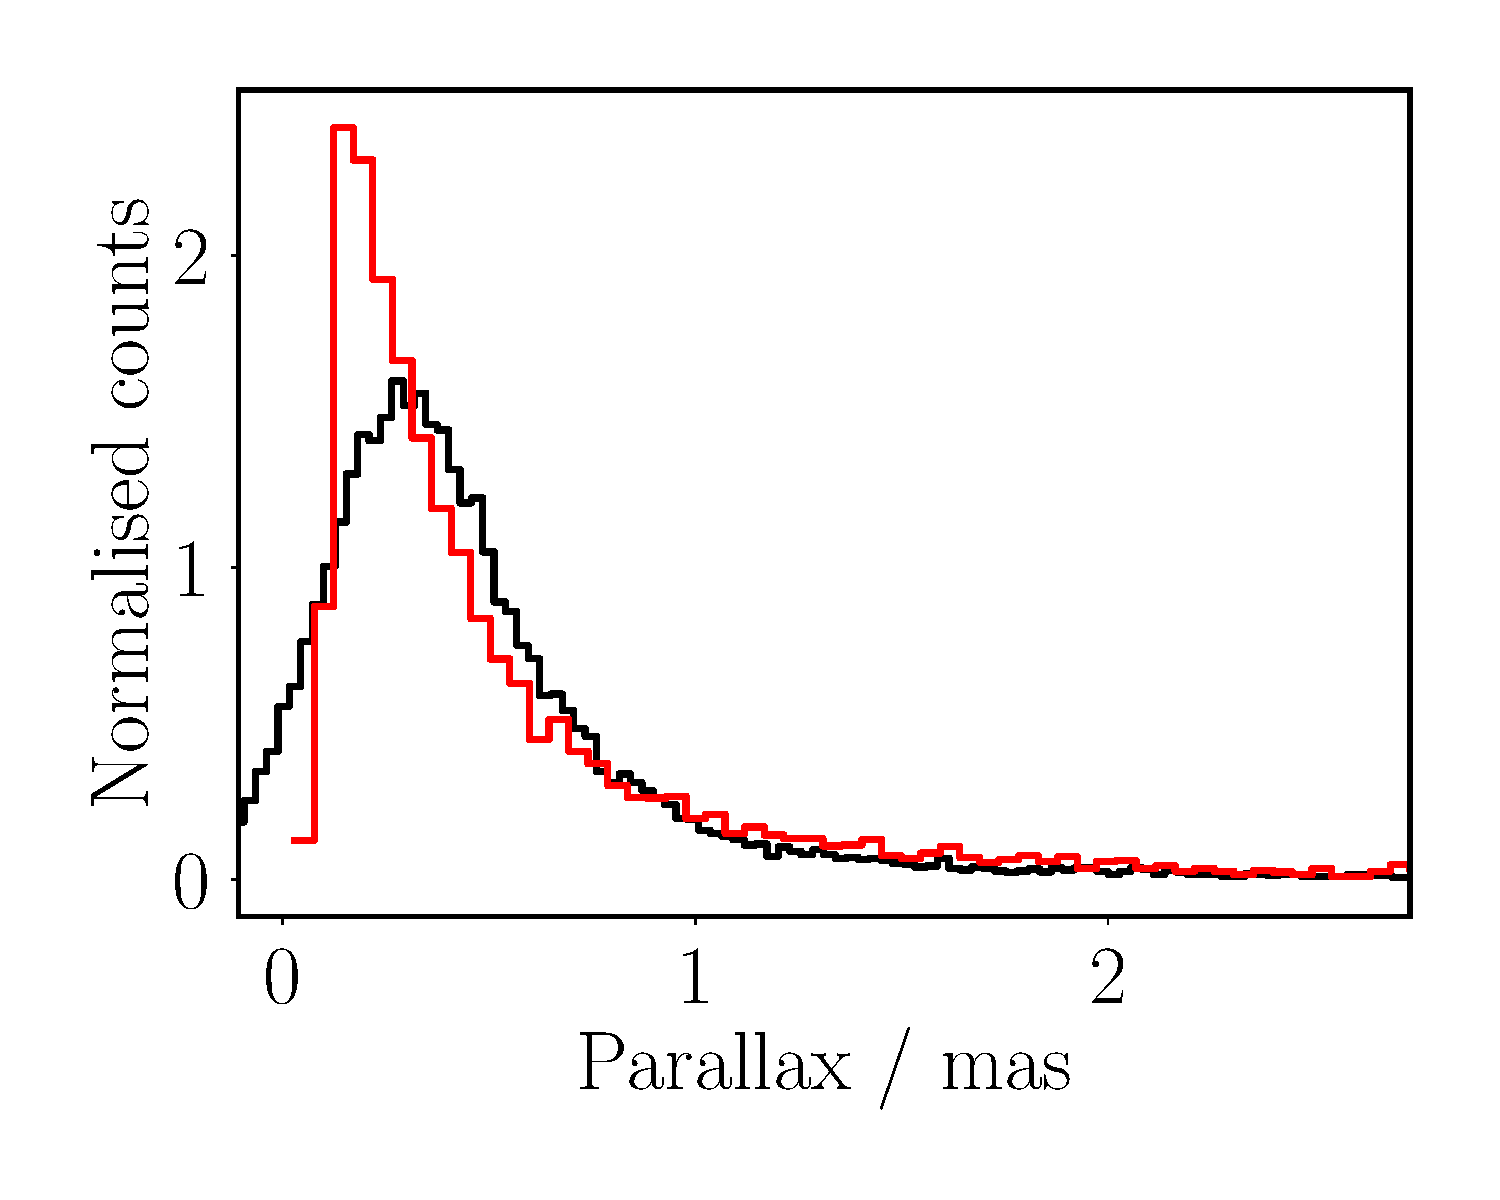
\includegraphics[width=\textwidth]{Plots/plot_dist_gaia_0_20_18.pdf}
        \caption{Parallaxes towards $l = 0^\circ$, $b = 20^\circ$.}
        \label{fig:l0dist}
    \end{subfigure}
    \begin{subfigure}[b]{0.3\textwidth}
        \centering
        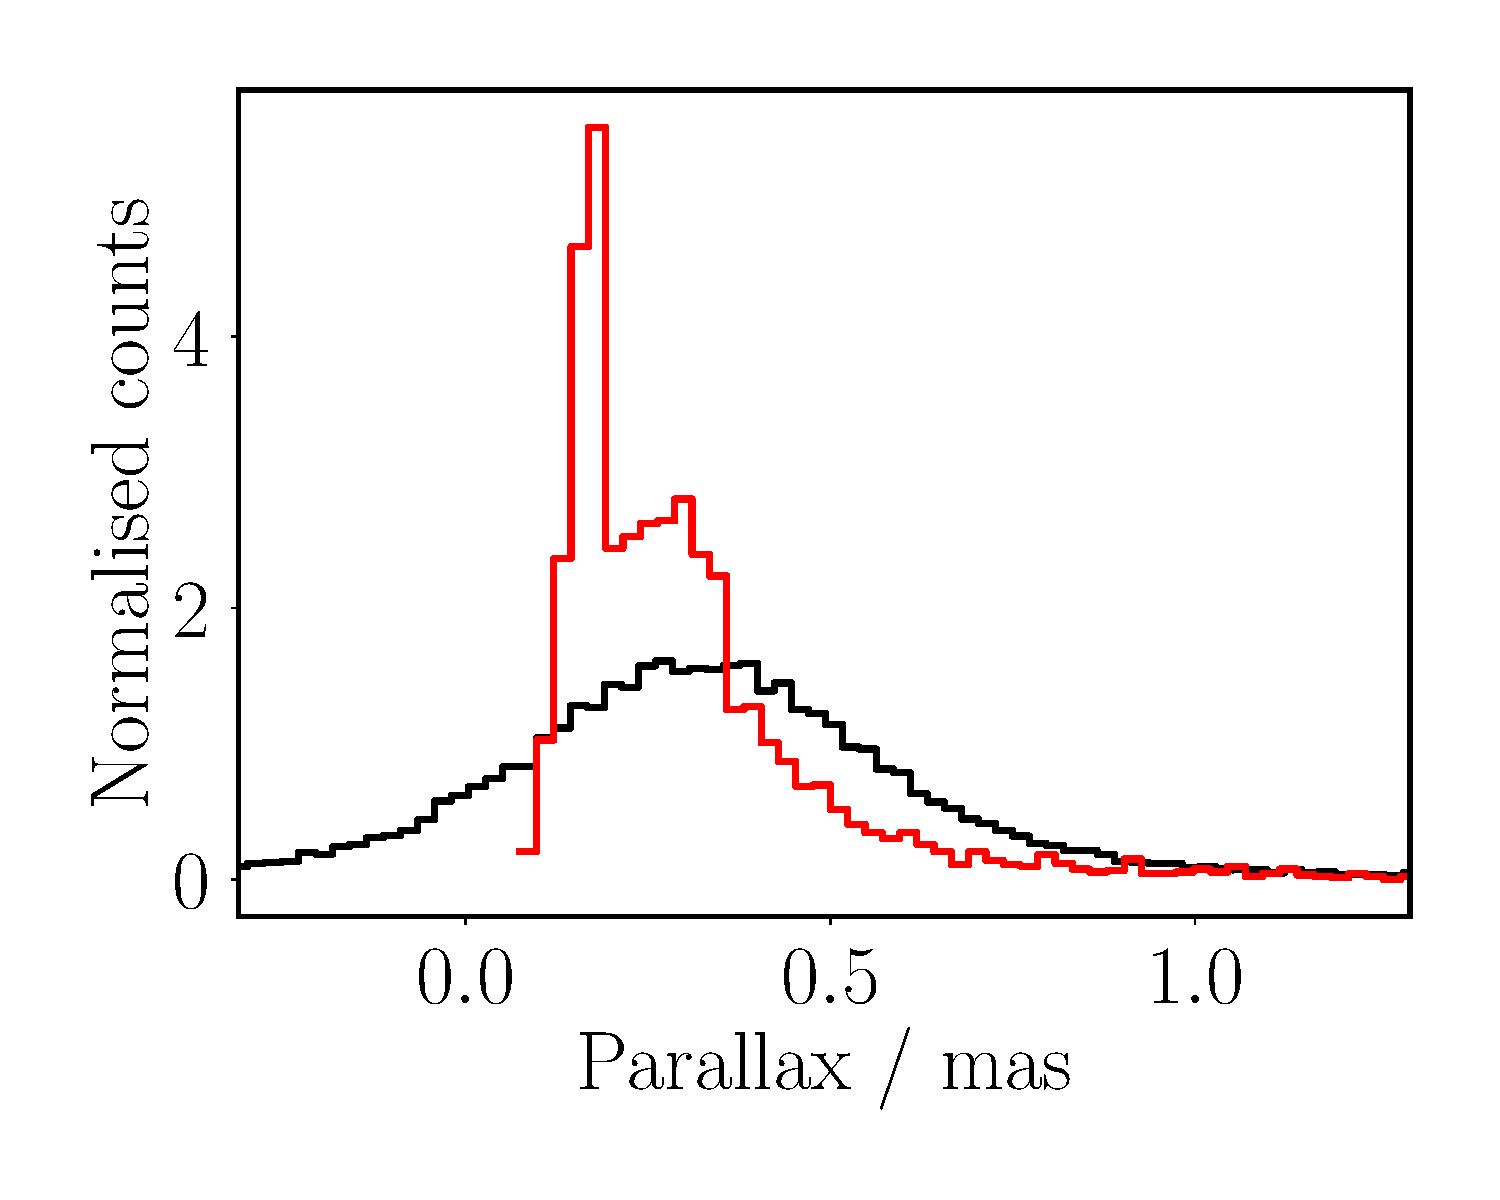
\includegraphics[width=\textwidth]{Plots/plot_dist_gaia_30_0_18.pdf}
        \caption{Parallaxes at $l = 30^\circ$, $b = 0^\circ$.}
        \label{fig:l30dist}
    \end{subfigure}
    \begin{subfigure}[b]{0.3\textwidth}
        \centering
        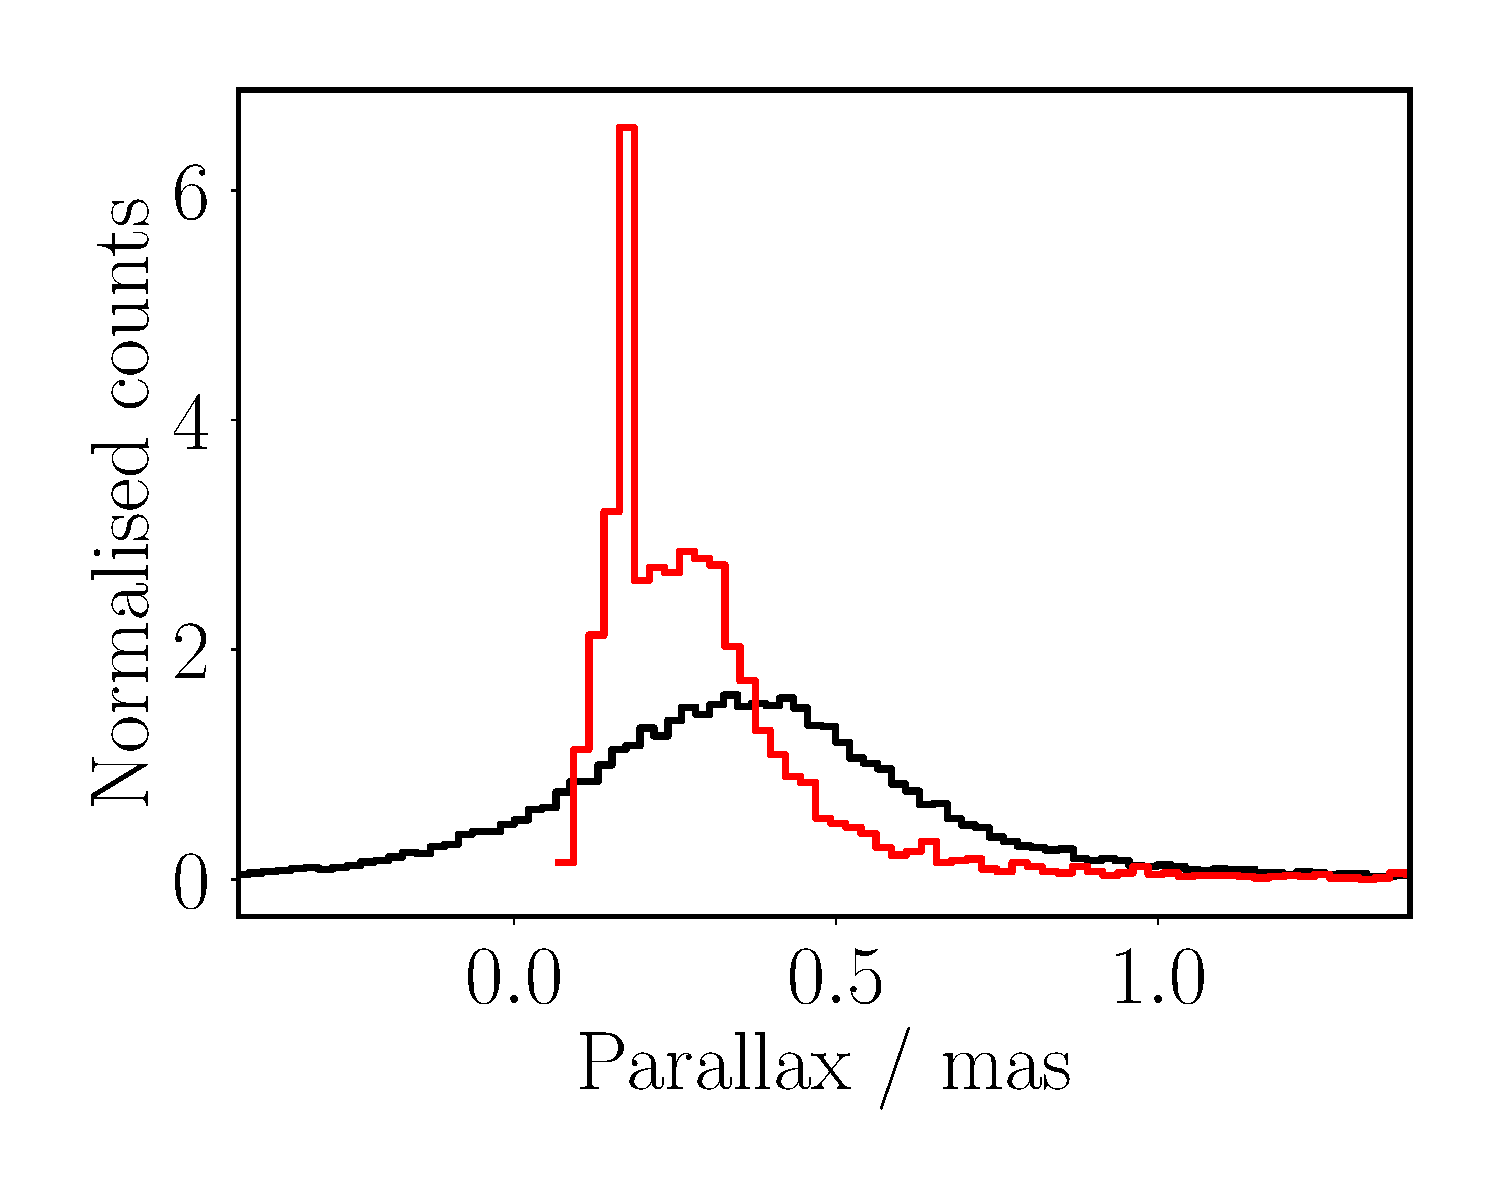
\includegraphics[width=\textwidth]{Plots/plot_dist_gaia_330_0_18.pdf}
        \caption{Parallaxes looking towards $l = 330^\circ$, $b = 0^\circ$.}
        \label{fig:l330dist}
    \end{subfigure}
    \caption{Distributon of measured parallaxes to sources towards the Galactic center; line colours and source samples are the as in Figure \ref{fig:goodishdists}.}
    \label{fig:badishdists}
\end{figure*}

This then leaves us with the three Galactic center sightlines, the two $y$ axis sightlines, and the two approximately Galactic anti-center sightlines to consider. We also get good agreement in the distribution of parallaxes for the Galactic anti-center (Figure \ref{fig:l180dist}); this distribution looks very similar to our $l = 220^\circ$ sightline, being roughly pointed away from the Galactic center and slightly out-of-plane. In the $y$ axis, the $l = 90^\circ$ and $l = 270^\circ$ directions, we get \textit{reasonable} agreement in our parallaxes, as shown in Figure \ref{fig:l90dist} for the $+y$ direction. Here we see a wider distribution of \textit{Gaia} parallaxes compared to the TRILEGAL data, with parallaxes spilling over into the unphysical (but mathematically allowed) negative values, but with similar distributions in their distributions to smaller distances (larger parallaxes).

Finally, we can examine the distribution of distances in the two samples of faint sources for the three Galactic center sightlines, as shown in Figures \ref{fig:l0dist}-\ref{fig:l330dist}. Here we start to see a breakdown in agreement between the distribution of parallaxes. The \textit{Gaia} data show a much broader distribution of parallaxes with an increase in negative values, with a much tighter distribution of inverse-distances in the TRILEGAL dataset.

Hence, we tentatively conclude that the large scale discrepancies we are seeing in some of our test sightlines is, in part, caused by selection biases with the two datasets. Here, \textit{Gaia} potentially suffer from selection bias, with more distance objects more systematically failing to derive a better-than-two-parameter solution during fitting -- although at $G = 18$ this effect will be small, perhaps no more than 2\% -- with parallaxes suffering from systematic biases, as well as the known \textit{Gaia} parallax zero-point offset. While the parallax signal-to-noise ratio for $G=12$ is as high as 100, it is of order 3 at $G=18$, and hence will suffer from several biases at such low SNRs. However, it is not clear naively how these distance biases, more obviously seen in the parallax data, affect the derived proper motions of a given source. The effect we see here is mirrored in other discussions of the potential pitfalls in using parallax data from \textit{Gaia}, such as Luri et al. (2018, A\&A, 616, A9, figure 10c).

Through either selection effect or systematic bias, we see that our sample of \textit{Gaia} sources in Figures \ref{fig:l0dist}-\ref{fig:l330dist} are smaller in distance from the Sun -- too large in parallax -- than the perhaps ``cleaner'' TRILEGAL distances (plus the broadening into negative parallaxes). Here we see that the $l = 0^\circ$ distribution is less affected than the two 30-degree-offset sightlines (Figure \ref{fig:l0dist} vs \ref{fig:l30dist} and \ref{fig:l330dist}), further correlating with the level to which our model and observed proper motions disagree. This would, if it were a selection effect, in turn, leave us with a collection of sources which are more affected by the Solar Motion, and hence a distribution of proper motions larger (in absolute sign) than our model distribution. In can, in fact, be seen in the $l = 330^\circ$ data (Figure \ref{fig:l330comp}) that there is a bimodality to the longitudinal proper motions for the faint sample, with a smaller subset of the data matching the TRILEGAL distribution in peak and shape towards zero proper motion. On the other hand, if this is a bias in the measured parallax, it will have an at present unknown effect on the proper motions. As discussed by Luri et al. this could be the so-called Lutz-Kelker bias (Lutz \& Kelker, 973, PASP, 85, 573), where the $d^2$ volume-based increase in the prior location for stars in the Galaxy mean they are more likely to have a true parallax smaller than its measured one than a larger true parallax.

At present we do not have a sufficiently robust explanation for this effect. We do not know whether the ``blame'' for the discrepancy lies with the \textit{Gaia} data or whether it is something we can -- or need to -- overcome if it is. We also do not know if the TRILEGAL simulation is simply failing to capture some astrophysics which would lead to our distances and hence proper motions being systematically wrong in the Galactic center. We also do not know if \textit{our} model is missing some crucial physics, or extra component of source motion in the Galaxy; we do not model the Galactic bulge, for example, stating that our distances should be within 5 kiloparsecs of the Sun, but these sources may have significant proper motions we do not capture.

\section{Conclusion}
We have derived here a simple model to describe the bulk motion of a random set of sources through the Galaxy. We project these motions to orthogonal proper motions, modelling the closed orbit of sources around the Galaxy, the Solar motion, and the random motions of the sources themselves. We compare this model to \textit{Gaia} sources in various sightlines across the Galactic plane -- in the mid-plane and slightly out of plane -- at different magnitude regimes to verify its robustness and accuracy.

Overall we find that our model matches the observed proper motions qualitatively -- quantitatively for bright sources, albeit aided by lower number statistics -- and hence are reasonably confident that our model is an acceptable description of the statistical proper motions of sources. This will be invaluable when matching the next generations of deep photometric surveys to one another, in the regime where \textit{Gaia} cannot provide individual proper motions for sources, without which we include a source separation bias which will impact the number of cross-matches reported between two such catalogues.

We find that our qualitative agreement between data and model breaks down in sightlines towards the Galactic center, but find this is likely rooted in discrepancies in the parallax of the two samples used to construct our data and model proper motions. The Galactic center sightlines suffer the most of all sightlines tested from poor parallax precision, or some bias in their determination, which correlates with proper motion disparity.

We are unable to disentangle whether this poor proper motion agreement in the Galactic center sightlines is caused by the \textit{Gaia} parallaxes influencing the corresponding proper motions, an issue with our TRILEGAL distances, some combination of the two, or some unknown source of proper motion independent of our parallaxes.  However, we are tentatively reassured that for the brighter sources, and in ``easier'' parts of the Galaxy, we obtain good agreement between our model and \textit{Gaia} proper motion offsets.

%%%%%%%%%%%%%%%%%%%%%%%%%%%%%%%%%%%%%%%%%%%%%%%%%%%%%%%%%%%%%%%%%%%%%%%%%%%%%%%%

\bibliographystyle{mnras}
\bibliography{../../../../LaTeX/postdoc_papers_jr2}



% Don't change these lines
\bsp	% typesetting comment
\label{lastpage}
\end{document}

% End of mnras_template.tex